\documentclass[11pt,a4paper]{article}

\usepackage{fullpage}
\usepackage[hidelinks]{hyperref}
\usepackage{graphicx}
\usepackage{wrapfig}
\usepackage{xargs}
\usepackage[pdftex,dvipsnames]{xcolor}
\usepackage{subcaption}
\usepackage{lipsum}

\usepackage{fancyhdr}
\pagestyle{fancy}
\fancyhf{}
\usepackage{todonotes}
\newcommandx{\change}[2][1=]{\todo[linecolor=red,backgroundcolor=red!25,bordercolor=red,#1]{#2}}
\newcommandx{\maybe}[2][1=]{\todo[linecolor=Plum,backgroundcolor=Plum!25,bordercolor=Plum,#1]{#2}}
\usepackage[utf8]{inputenc}

\renewcommand{\headrulewidth}{0pt}
\renewcommand{\footrulewidth}{0pt}

\fancypagestyle{firstpagefooter} {
	\lfoot{\tiny{Version: 25.09.2018}}
	\cfoot{}
	\rfoot{\thepage}
	
}

\lfoot{Name: Doruk Çetin - Legi: dcetin - Student Number: 18-947-382}
\rfoot{\thepage}

\begin{document}

\title{Advanced Systems Lab Report\\ \normalsize{Autumn Semester 2018}}
\author{Name: Doruk Çetin\\Legi: dcetin\\Student Number: 18-947-382}
\date{
	\vspace{4cm}
	\textbf{Grading} \\
	\vspace{0.5cm}
	\begin{tabular}{|c|c|}
		\hline  \textbf{Section} & \textbf{Points} \\
		\hline  1                &                 \\ 
		\hline  2                &                 \\ 
		\hline  3                &                 \\ 
		\hline  4                &                 \\ 
		\hline  5                &                 \\ 
		\hline  6                &                 \\ 
		\hline  7                &                 \\ 
		\hline \hline Total      &                 \\
		\hline 
	\end{tabular} 
}
\maketitle
\thispagestyle{firstpagefooter}

\newpage

\section{System Overview} \label{sec:overview}
Aim of the middleware is to collect and forward queries from clients to servers, wait for the responses and reply the clients back — all under specified conditions and configurations. Aforementioned servers and clients are the single-threaded instances of Memcached \cite{memcached} and of memtier\_benchmark \cite{memtier}, respectively. The design of the middleware spans several classes and functions that implement different functionalities. The classes operate in a multithreaded fashion so the different functionalities can work together asynchronously.

\subsection{System Design} \label{sec:ov-system-design}
\begin{figure}[h]
  \centering
  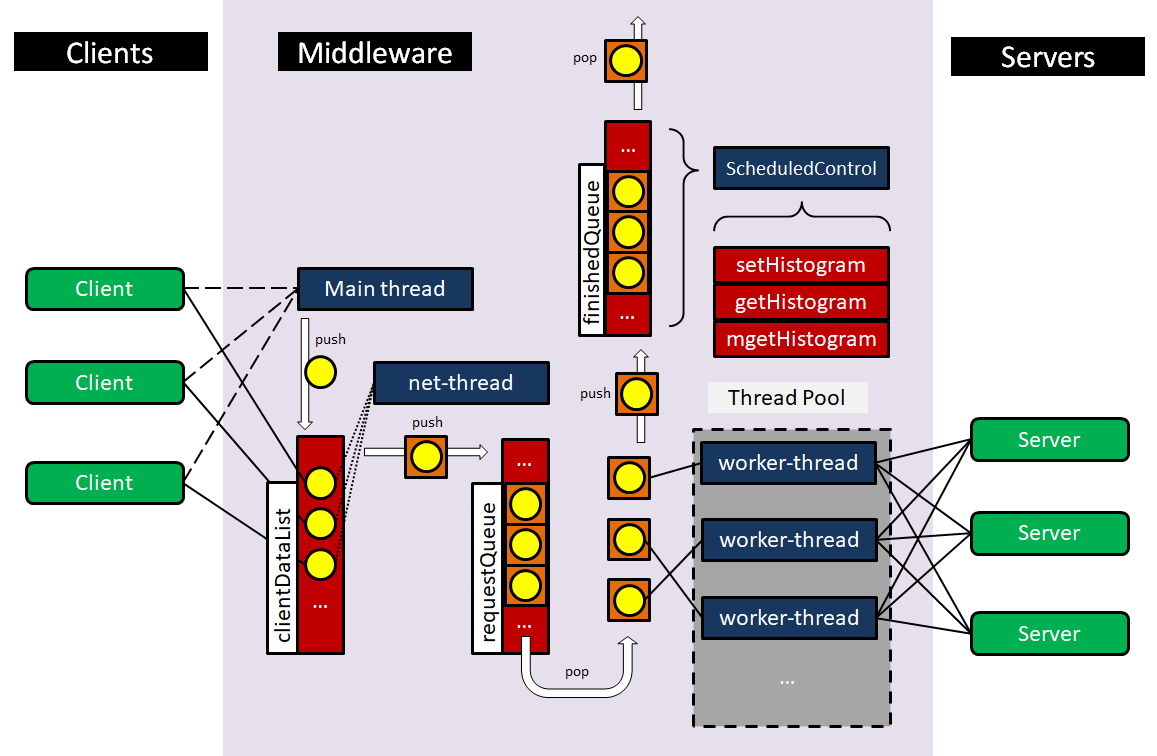
\includegraphics[width=0.7\linewidth,trim={0px 0px 0px 0px},clip]{img/system-diagram.png}
  \caption{A simplified diagram of the system showing the inner structure of the system and the interaction of its components in an informal manner. Circles represent the clientData objects and the squares represent the requestData objects, whose instances encapsulate the ones of the former. Dark gray rectangles represent the threads in the system, of which there are always three plus the size of the worker thread pool. Light gray rectangles represent the shared lists, of which there are three as shown. Light gray rounded rectangles illustrate the external systems, namely the clients and servers. Dashed line shows the communication with the welcomingSocket and the dotted line is net-thread checking if there is any request available. Solid lines represent the main information flow from clients to servers and again back to the clients.}
  \label{fig:system-diagram}
\end{figure}

\subsubsection{Main thread} \label{sec:overview-mainthread}
Main thread of the \underline{MyMiddleware} class is responsible for setting up the working environment for the whole system. It first initializes the shared data structures that are to be used by other threads; namely, these are \underline{clientDataList} (which stores information about each one of the connected clients), \underline{requestQueue} (which is a first-in, first-out queue for queries awaiting execution) and \underline{finishedQueue} (which temporarily stores the completed requests for the aggregation of their statistics). It then creates a \underline{clientHandler} (so-called "net-thread", which is responsible for handling communication with clients) and the specified number of \underline{serverHandler} threads (so-called "worker-threads", which are responsible with for handling communication with the servers). Throughout this report, names clientHandler and net-thread will be used interchangeably. Same also applies for worker-threads and serverHandlers. Lastly, the main thread creates the \underline{welcomingSocket} and listens for incoming client connections in a loop. As soon as such a connection request is received, main thread creates the respective \underline{clientData} object and pushes it into the clientDataList.
\par
clientData objects store the information relevant for communicating with the clients. They consist of the net socket, its respective reader and writer streams, an identifier number and lastly a flag that denotes if the client has already sent its request and awaiting for reply.

\subsubsection{clientHandler (net-thread)} \label{sec:ov-netthread}
The clientHandler constantly iterates over the clientDataList, waiting for new requests from clients. It employs busy waiting as it non-blockingly check each client to see if there is an available request. As soon as it receives its first query from a client, clientHandler initializes the \underline{ScheduledControl} thread, which is responsible for periodically aggregating statistics of the system. clientHandler checks for each client if it has not been waiting for a repy and data is available in its reader stream. That means that client has a new request so the clientHandler creates a new \underline{RequestData} object and pushes it into the requestQueue for it to be handled by the worker-threads.
\par
At the beginning of each iteration over the clientDataList, clientHandler compares the time with the timestamp of the last received query. If it is larger than some safe threshold, that means no other requests will arrive for our working conditions, so it moves on to close the system killing all threads. Before exiting clientHandler prints the response time histogram created by the ScheduledControl thread.
\par
requestData objects contain the necessary relevant information about a request so that it can be executed correctly and its statistics can be aggregated with ease. Aside from information about its respective client, it stores an identifier number, the type of the request (set, get or multi-get), which server the request is sent to (if it is a get or multi-get request), which worker-thread handled the request, how many items were requested and received (if it is a get or multi-get request) and its timestamps.
\par
Timestamps are all kept in nanoseconds. \underline{ns\_netThreadReceived} marks the time net-thread received the request from the client. \underline{ns\_workerThreadReceived} marks the time the request has exited the request queue to be handled by a worker-thread. The difference of those two timestamps give the \textbf{waiting time in the queue}. Lastly, there is \underline{ns\_workerThreadFinished} that marks the worker-thread received an answer from the servers (either successful or not) and replied to the querying client for the request. The difference of this last two timestamps (namely ns\_workerThreadFinished and ns\_workerThreadReceived) gives the \textbf{service time of the memcached servers}. The terms queueing time and waiting time in the discussions that take place in the later sections refer respectively to waiting time in the queue and the service time of the memcached servers.

\subsubsection{serverHandlers (worker-threads)} \label{sec:ov-workerthread}
serverHandler threads initially set up dedicated connections to each server with their reader and writer streams. They also operate in an infinite loop, waiting for new request to take from the requestQueue in a blocking manner. It is blocking as a worker thread has no other jobs than handling requests. As soon as there is an available request in the queue the worker-thread wakes up, marks the time and unpacks the requestData structure. Worker-threads are the ones that parse the messages, so the certain specifics of the requests are unknown to the system until they exit the queue. After it has been handled accordingly to its type, the resulting requestData is pushed into the finishedQueue.
\par
If it is a set query, the request is sent to all of the servers and reported as successful to the client only if all the responses indicate so. If not, one of the error messages are relayed to the sender client. If it is a get request there are two possibilities. If it is a multi-get request in a multi-server setting with \texttt{readSharded} option provided as true, then it is sharded into smaller requests. If the query requests a single object, there is a single server or \texttt{readSharded} is provided as false, then the request will be sent to only one server. In either case, middleware employs a simple load balancing scheme through a round-robin scheduling. It iterates over all servers while sending get requests or the sharded get requests. For both set and get requests middleware first sends the requests to servers and then collect the responses. Middleware outputs for the later experiments confirm that thw workload is indeed distributed equally to multiple servers, as seen on Figure\ref{fig:equal-load}.

\begin{figure}[h]
\centering
\begin{subfigure}{.33\textwidth}
  \centering
  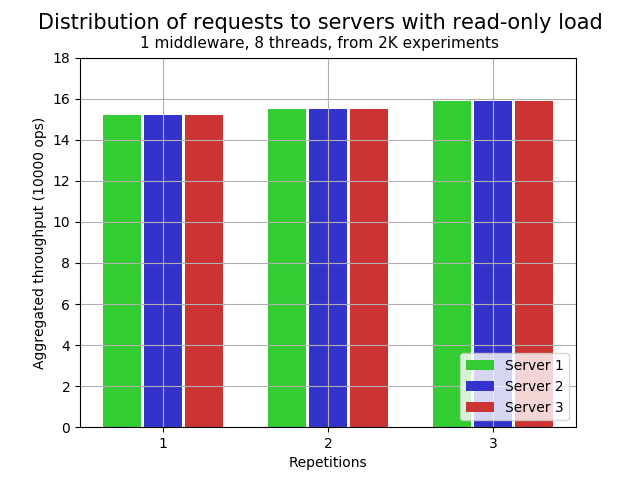
\includegraphics[width=1.0\linewidth,trim={0px 0px 0px 0px},clip]{img/plot/equal-load-read-only.png}
  \caption{Read-only load}
  \label{fig:equal-load-read-only}
\end{subfigure}%
\begin{subfigure}{.33\textwidth}
  \centering
  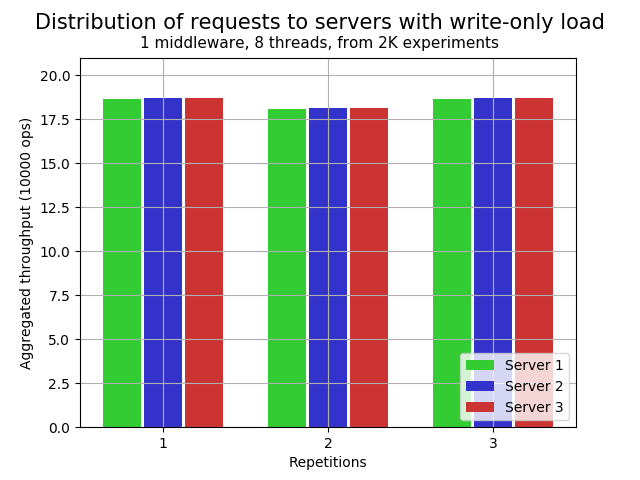
\includegraphics[width=1.0\linewidth,trim={0px 0px 0px 0px},clip]{img/plot/equal-load-write-only.png}
  \caption{Write-only load}
  \label{fig:equal-load-write-only}
\end{subfigure}%
\begin{subfigure}{.33\textwidth}
  \centering
  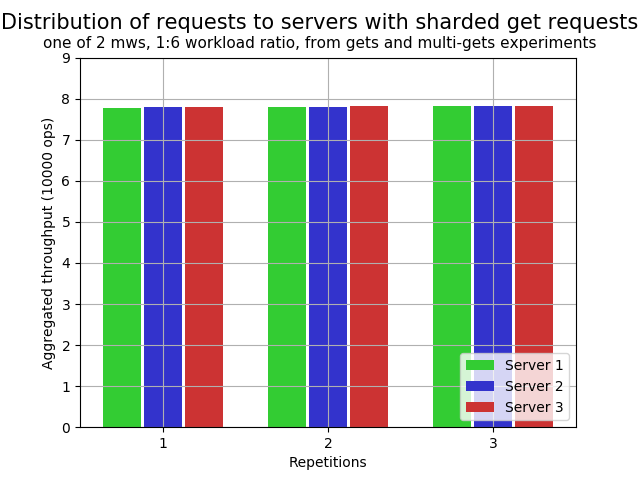
\includegraphics[width=1.0\linewidth,trim={0px 0px 0px 0px},clip]{img/plot/equal-load-sharded-get.png}
  \caption{Sharded get requests}
  \label{fig:equal-load-sharded-get}
\end{subfigure}
\caption{Distribution of the requests to three servers over three repetitions. Each of the plots illustrate a different workload condition. Results are taken from the experiments of later sections. Figures \ref{fig:equal-load-read-only} and \ref{fig:equal-load-write-only} use the results from 2K experiments \ref{sec:2k} and Figure \ref{fig:equal-load-sharded-get} use those from gets and multi gets experiments \ref{sec:gmg}}
\label{fig:equal-load}
\end{figure}

\subsubsection{ScheduledControl} \label{sec:ov-scheduledcontrol}
ScheduledControl is started by the net-thread as it receives its first request. It periodically wakes up, aggregates the new information, then sleeps again. It goes over the entries in finishedQueue in its each run, collecting type-specific statistics. ScheduledControl keeps track of the distribution of the response times for different types of requests by constructing a separate histogram for each type of request, namely sets, gets and multi-gets. While going over the list of requests the ScheduledControl assigns each of the requests to the appropriate histogram bin with respect to its response time and type. Additionally, length of the requestQueue is saved in each run of the ScheduledControl.

\subsubsection{Internal parameters} \label{sec:ov-internalparameters}
The system has several options hardcoded as parameters of MyMiddleware class:
\begin{itemize}
\item \texttt{verboseLogs} specifies if the system should output the work logs or not. Such logs are printed when a request is received, relayed to servers, got answered and replied back to the clients. It also prints out details about which thread handled the request, which client sent the request, to which server the request was sent to and the completely parsed messages and replies. It is a useful option for understanding the inner workings and state transitions of the middleware system. It should be set as false if user is not debugging.
\item \texttt{verboseAggr} controls the outputting of the aggregated statistics. It is always true for our experiments as it is our main tool for analysing the system.
\item \texttt{timeoutSecs} specifies the amoun of time the system should wait until new queries before shutting itself down. Altough the middleware can work seamlessly without any interruption, systems needs to be restarted to operate in its most efficient manner in its current implementation. 3 seconds are proved to be enough for our experiments.
\item \texttt{initDelaySecs} and \texttt{periodSecs} respectively specify the initial delay and the period of the ScheduledControl runs. Both are given as 1, that means the ScheduledControl thread begins collecting data after an initial delay of 1 seconds and it wakes itself at the end of every 1 second period after that.
\item \texttt{sep} sets the column separator to be used by ScheduledControl when outputting aggregated statistics. We output the aggregation table inside the output file in a comma separated format, so we set sep as \texttt{','}.
\end{itemize}

\subsection{Methodology} \label{sec:ov-methodology}
\begin{table}
\begin{minipage}{.5\textwidth}
	\centering
	\begin{tabular}{|l|c|}
		\hline Number of servers                & nsvr		\\
		\hline Number of client machines        & ncli		\\
		\hline Instances of memtier per machine & icli		\\
		\hline Threads per memtier instance     & tcli		\\
		\hline Virtual clients per thread       & vcli		\\
		\hline Workload                         & wrkld		\\
		\hline 
	\end{tabular}
\end{minipage}%
\begin{minipage}{.5\textwidth}
	\centering
	\begin{tabular}{|l|c|}
		\hline Multi-Get behavior               & mgshrd	\\
		\hline Multi-Get size                   & mgsize	\\
		\hline Number of middlewares            & nmw		\\
		\hline Worker threads per middleware    & tmw		\\
		\hline Repetitions                      & reps		\\
		\hline Test time                        & ttime		\\
		\hline 
	\end{tabular}
\end{minipage}
\caption{Abbreviations for experiment parameters.} \label{tab:param-abbrs}
\end{table}
All the necessary commands for initializing the experimental setup and conducting the experiments are provided in a companion file called \texttt{commands.sh}. It also exemplifies the usage of auxiliary technologies used for further analysing the system and its environment as well as it contains some other helpful commands for copying and plotting the experiment results. \texttt{plot} folder contains all scripts (and their eventual outputs) necessary for plotting the results placed under the \texttt{res} folder. Every plot provided inside or alongside this report is reproducible with the provided data and the scripts. \change{Probably should detail which scripts correspond to which experiments and how the results should be placed.}Lastly, \texttt{runner.sh} is the encapsulating script that runs the desired agent (i.e. client, middleware, server or dstat \cite{dstat} tool) for the configuration provided through the command line arguments. The arguments it expects share the same nomenclature we use	in scripts to refer the experiment parameters. Here, in Table \ref{tab:param-abbrs}, we list these abbreviations. Result directory hierarchy also obeys the same nomenclature.
\par It is important to pay attention the order and timing of executing commands. Servers should be run first and the middlewares (if any) should start waiting connections. Then, both the clients and dstat processes should start simultaneously — we could do this by using Cluster SSH (also called as cssh) \cite{cssh}. Clients, middlewares and dstat processes ran accordingly for three separate repetitions, afterwards they should be restarted by hand. Another important thing to keep in mind while using the project codebase is to remember that the codes do not cover erroneous cases. For example, middleware does not support any other operations than set or get. Similarly, plotting scripts may not work with data with erroneous content, filenames, directory hierarchy and such.
\\
\par Three repetitions were seem to be sufficient all the experiments as both our middleware and the external systems it communicated had shown performances that stayed fairly stable under repetitions. Similarly, trimming five seconds of warm-up and cool-down periods, respectively at the beginning and the end of experiments, was found as sufficient through the initial exploratory experiments performed. Clients can lag behind around at most one second per a three repetition run, but it is still negligible with the times cut for warm-up and cool-down periods. Baseline without middleware expriments (Section \ref{sec:csb}) were run for 100 seconds per each iteration, yielding a one and a half minute period after cutting the warm-up and cool-down times. Experiments involving middleware (Sections \ref{sec:mwb}, \ref{sec:tpfw}, \ref{sec:gmg} and \ref{sec:2k} consists of three repetitions of 70-second runs yielding a 60 second stable period for aggregation.
\par iPerf3 \cite{iperf} is used to measure the maximum achievable bandwith in between different machines in our environment. For each machine in every experiment, we collect data through dstat. dstat is run in its default mode, so it collects statistics cpu, disk, network, paging and system  statistics. It collects data every second after an initial delay of one second — similar to the ScheduledControl in our middleware.
\\
\par Error bars in plots show a range of one standard variance, unless indicated otherwise. Most of the plots have their x-axis as the number of clients. It is the effective number of different clients and is simply calculated by multiplying four numbers: number of virtual clients per thread, number of threads per memtier instance, number of memtier instances per virtual machine and the number of client machines. Using the abbreviations in Talbe \ref{tab:param-abbrs} the formula could be written as $numClients = vcli \times tcli \times icli \times ncli$. The term latency is used interchangeably with the term response time. Plots specify the source of measurements as middlewares or clients in their subtitles, so it is easy to find for a plot whose perspective it reflects.
\par For every experiment, interactive law is verified by both calculating the throughput from the response times and vice versa. As it would approximately double all the plots we provide here to show that the interactive law indeed holds for all the experiments, we only provide the illustration of this guarantee in Section \ref{sec:csb}. Figures \ref{fig:csb1-wo-law}, \ref{fig:csb1-ro-law}, \ref{fig:csb2-wo-law} and \ref{fig:csb2-ro-law} show the actual and predicted values coincide perfectly. Reader should feel free to run the provided scripts for other experiments and see the interactive law in action in other experiments as well.
\\
\par In  experiments involving the get operations the servers are always populated beforehand so miss rates are either realistic and negligible. Server population is always done in the same manner: first 99\% of the keys that are to be used in experiments were set by the sequential load option of the memtier. Therefore, for all the get requests we expect similar miss rates which are around 1\%. Some actual miss rates, from the baseline with middleware experiments, can be viewed in Section \ref{sec:mwb-summary}.


\section{Baseline without Middleware} \label{sec:csb}
In this section, we examine the characteristics of the clients and servers before the introduction of the middleware to the environment. For all different configurations of different experiments we show that the interactive law holds true by calculating the throughput values from the response times and vice versa. Values predicted through the interactive law are always illustrated alongside the actual values obtained by the memtier outputs.

\subsection{One Server} \label{sec:csb1}
First setting contains three memtier clients connecting to one memcached server. Each of the client machines has one memtier instance with two client threads running in them. We vary the number of virtual clients and the type of workload (write-only and read-only) and observe the change in the performance of the system.

\begin{figure}[h]
\centering
\begin{subfigure}{.5\textwidth}
  \centering
  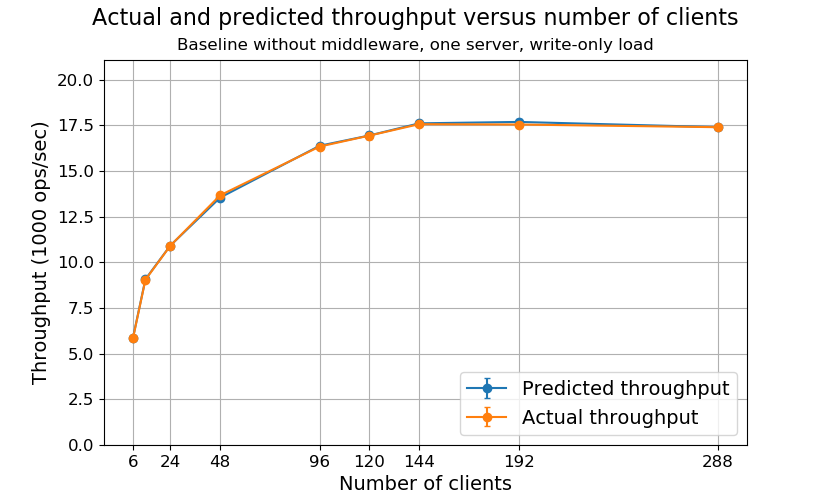
\includegraphics[width=1.0\linewidth,trim={0px 0px 0px 0px},clip]{img/plot/csb1-wo-law_tpt.png}
  \caption{Write-only throughput}
  \label{fig:csb1-wo-law_tpt}
\end{subfigure}%
\begin{subfigure}{.5\textwidth}
  \centering
  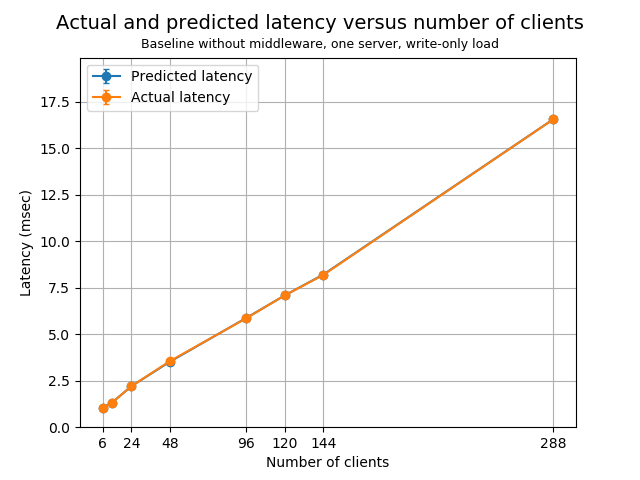
\includegraphics[width=1.0\linewidth,trim={0px 0px 0px 0px},clip]{img/plot/csb1-wo-law_lat.png}
  \caption{Write-only latency}
  \label{fig:csb1-wo-law_lat}
\end{subfigure}
\caption{Throughput and latency values for the write-only workload for baseline without middleware, for one server case.}
\label{fig:csb1-wo-law}
\end{figure}

\begin{figure}[h]
\centering
\begin{subfigure}{.5\textwidth}
  \centering
  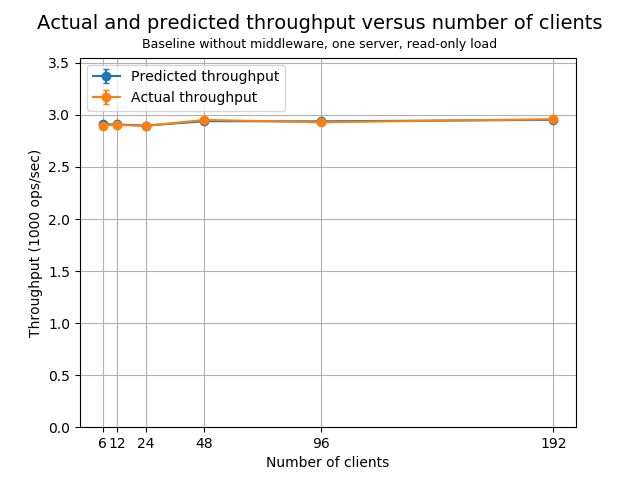
\includegraphics[width=1.0\linewidth,trim={0px 0px 0px 0px},clip]{img/plot/csb1-ro-law_tpt.png}
  \caption{Read-only throughput}
  \label{fig:csb1-ro-law_tpt}
\end{subfigure}%
\begin{subfigure}{.5\textwidth}
  \centering
  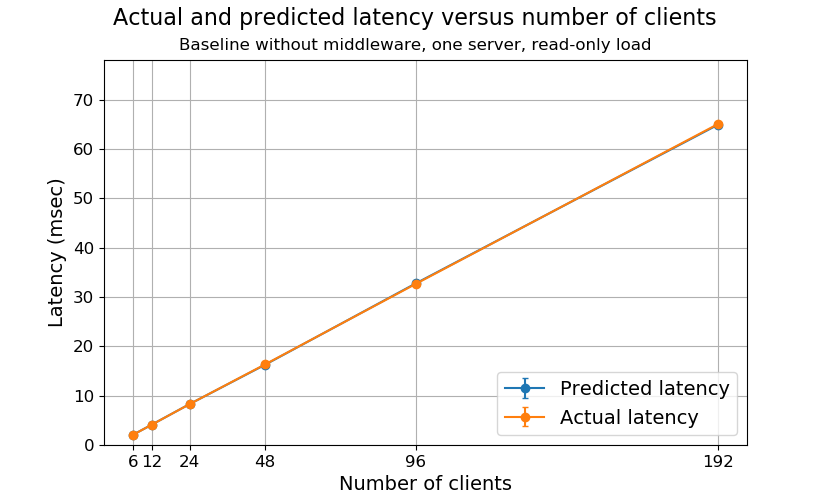
\includegraphics[width=1.0\linewidth,trim={0px 0px 0px 0px},clip]{img/plot/csb1-ro-law_lat.png}
  \caption{Read-only latency}
  \label{fig:csb1-ro-law_lat}
\end{subfigure}
\caption{Throughput and latency values for the read-only workload for baseline without middleware experiment with one server case.}
\label{fig:csb1-ro-law}
\end{figure}

\subsubsection{Explanation} \label{sec:csb1-exp}
We see the results for the one server configuration in Figures \ref{fig:csb1-wo-law} and \ref{fig:csb1-ro-law}. Plots show that the interactive law holds true for both experiments.

\par For the write-only part, we can observe the systems starts as undersaturated and saturates around 144 clients by looking at the values of both plots. Throughput increases steadily until the saturation point, as additional clients are connected to the system. Afterwards we cannot observe even marginal increases in the throughput. We see a similar trend in the response time plot as it is slightly curved until around the saturation point but linear afterwards. After the saturation point, the systems cannot handle any more requests and the average response time increases linearly with respect to number of clients while there is no increase in throughput values as the system is already at full capacity.
\par The reason behind this saturation is meeting the network bandwidth capacity. dstat files show that each client can send at most 24MB per second on average. Looking at the iperf results we can see that client to server communication is limited by 24MB per second for different configurations. As we send 4096B data that means we can send $\sim 6000$ requests per machine, $\sim 18000$ requests in total, and this corroborates our results.\maybe{is usage limited by correct, both here and below?}

\par In the read-only part, we see that the system begins operating in the overly-saturated region for the minimum number of clients we can achieve, which is 6. We conclude this as we cannot observe any noticeable change in throughput when we vary the number of clients and the response time is approximately a linear function of the number of clients everywhere. Although we can see the absolute maximum of the throughput plot is at 32 clients, it is clear that the system becomes highly inefficient with the addition of each additional client to the system after 6 clients. Only increases in the throughput are quite marginal whereas response times double when we double the number of clients in the system.
\par Again, dstat and iperf together confirm our assertions and indicates the reason for the saturation. iperf states the server to client connection is limited by 12MB per second and it is what we observe in our server for varying number of clients through all repetitions. This implies the server can reply to at most $\sim 3000$ requests per second and it is in line with our results.

\subsection{Two Servers} \label{sec:csb2}
This configuration deals with one client machine sending requests to two servers. This time the client machine has two instances of memtier running (each connected to a different server) with one client thread per instance. We again change the workload (write-only and read-only) and change the total number of clients by varying the virtual number of clients and observe the changes in the performance.

\begin{figure}[h]
\centering
\begin{subfigure}{.5\textwidth}
  \centering
  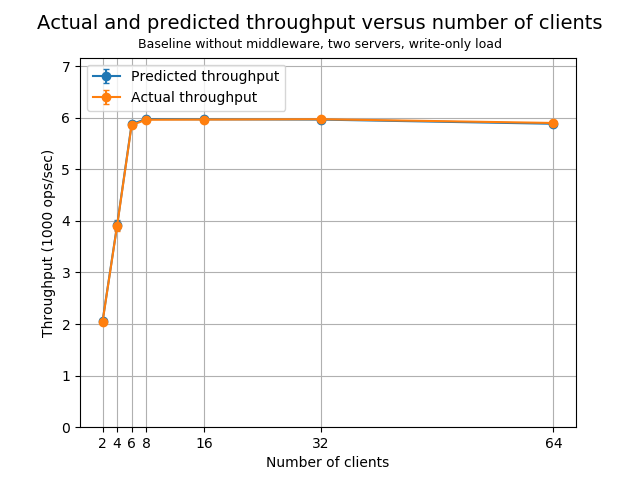
\includegraphics[width=1.0\linewidth,trim={0px 0px 0px 0px},clip]{img/plot/csb2-wo-law_tpt.png}
  \caption{Write-only throughput}
  \label{fig:csb2-wo-law_tpt}
\end{subfigure}%
\begin{subfigure}{.5\textwidth}
  \centering
  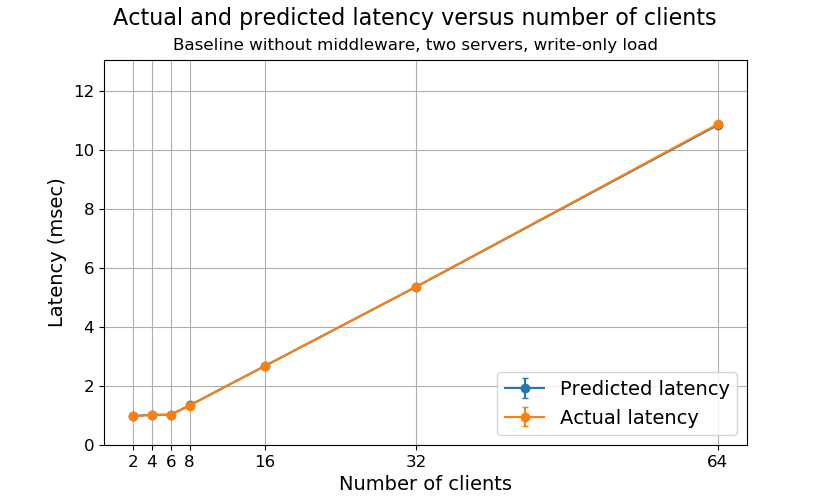
\includegraphics[width=1.0\linewidth,trim={0px 0px 0px 0px},clip]{img/plot/csb2-wo-law_lat.png}
  \caption{Write-only latency}
  \label{fig:csb2-wo-law_lat}
\end{subfigure}
\caption{Throughput and latency values for the write-only workload for baseline without middleware experiment with two servers.}
\label{fig:csb2-wo-law}
\end{figure}

\begin{figure}[h]
\centering
\begin{subfigure}{.5\textwidth}
  \centering
  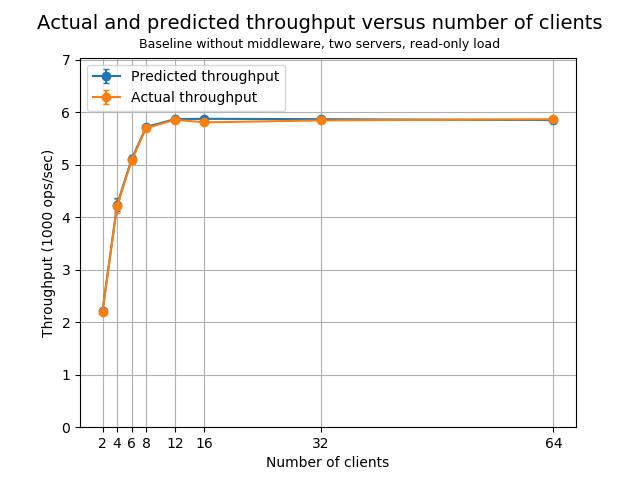
\includegraphics[width=1.0\linewidth,trim={0px 0px 0px 0px},clip]{img/plot/csb2-ro-law_tpt.png}
  \caption{Read-only throughput}
  \label{fig:csb2-ro-law_tpt}
\end{subfigure}%
\begin{subfigure}{.5\textwidth}
  \centering
  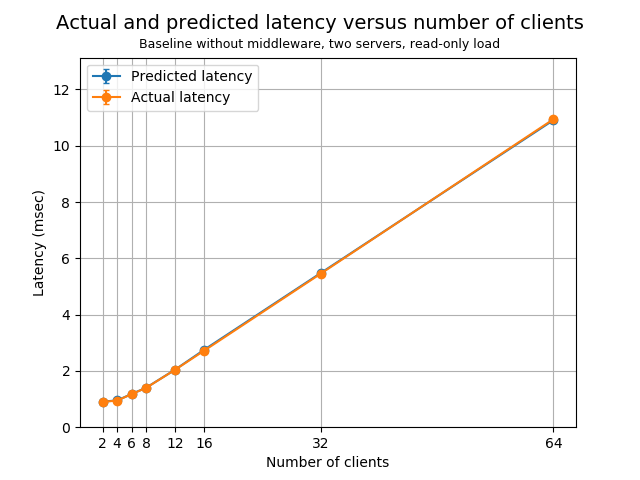
\includegraphics[width=1.0\linewidth,trim={0px 0px 0px 0px},clip]{img/plot/csb2-ro-law_lat.png}
  \caption{Read-only latency}
  \label{fig:csb2-ro-law_lat}
\end{subfigure}
\caption{Throughput and latency values for the read-only workload for baseline without middleware experiment with two servers.}
\label{fig:csb2-ro-law}
\end{figure}

\subsubsection{Explanation} \label{sec:csb2-exp}
Results are illustrated in Figures \ref{fig:csb2-wo-law} and \ref{fig:csb2-ro-law}. Unlike the first part, we obtain similar plots for both the read-only and the write-only case. We say that the system saturates when there is 8 clients in the system for both cases, as it is elbow point for the throughput plots and the response time values continue increasing linearly after crossing 8 clients. We can clearly say that the system is under saturated before those points as the throughput rises quickly we only see marginal changes in the response times in both workloads.
\par The main reasons behind the saturation for both cases are the same: the network bandwith limitations. Although interestingly, the write-only and read-only cases have their bottlenecks in different parts of the network pipeline. Situtation is quite similar to the earlier results in Section \ref{sec:csb1}. For the write-only case, dstat outputs for the saturated configurations show that the client sends at most 24MB per second to servers, which is its limit confirmed by iperf statistics. This corresponds to a total of $\sim 6000$ requests distributed to two servers, corroborating our results. We also know through iperf that a server can send at most 12MB per second and and we see the same numbers in our dstat files for the read-only part. This equals to 24MB per second received by clients, again amounting to a total of $\sim 6000$ requests, this time as a result of another limiting factor. As a bottom line, both configuration saturating around 8 clients is a coincidental outcome of the bandwidth parameters since one configuration is limited by the client side whereas the other is limited by the server side.

\subsection{Summary} \label{sec:csb-summary}
Here, we comparatively analyse the different results for the previously discussed set of experiments. The results are explained in more detail in Sections \ref{sec:csb1-exp} and \ref{sec:csb2-exp}, so we will not be going into the specifics of each experiment here.
\begin{table}[h]
\small
\centering
{Maximum throughput of different VMs.}
\begin{tabular}{|l|p{2.1cm}|p{2.2cm}|p{6cm}|}
\hline 	                      & Read-only workload & Write-only workload & Configuration gives max. throughput \\ 
\hline One memcached server & $2897.9 \pm 16.4$ & $17556.5 \pm 50.1$ & read-only: 6, write-only: 144 clients \\ 
\hline One load generating VM & $5698.5 \pm 27.2$ & $5960.9 \pm 3.2$   & both workloads: 8 clients \\ 
\hline 
\end{tabular}
\caption{Summary of baseline without middleware experiments.} \label{tab:csb-summary}
\end{table}
\par Table \ref{tab:csb-summary} reports the maximum throughput obtained in both experiments and the configurations that allow such maxima. For both experiments under either read-only or write-only workload conditions, we have concluded that the bottleneck of the system is always the network bandwidth. Intuitively enough, write-only requests have large queries and small responses as they send the data to be stored and only return with a confirmation or an error message. The situation is reversed for the read-only workload as get requests merely contain the keys but their replies carry the data itself (as we get a hit rather than a miss almost everywhere). Therefore, it is in line with our expectations that the throughput values for the experiments with write-only workload are limited by the client to server bandwidth and similarly, throughput values for the read-only counterparts are limited by the server to client bandwidth. These arguments apparently reflect on our results in Table \ref{tab:csb-summary}. 
\par Read-only throughput doubles as we introduce another server to our one server setting. Similarly for the write-only workload, by going from three load generating machines to a one client setting we can see expect the throughput to become one third of what it was before.
\\
\par As a side note, we observe only the write-only workload with three client machines resulting a high percentage of CPU usage in servers, in the saturated region. The idle time of the server for this setting is under $20\%$ most of the time. Aside from this specific case not one server or client experience any high CPU utilization, idle times are consistently above $90\%$.
\par It is also worth noting that for the read-only workload in one server setting (Section \ref{sec:csb1-exp}) we state the system is overly-saturated rather than saturated with the presence of 6 clients, even though we do not have any information regarding the fewer number of clients. It is the outcome of a comparison with the read-only experiments with two servers and one client, as we notice that with 6 clients on client machine can help achieve a throughput around 2000 requests. Keeping in mind that the server performance is not a bottleneck anywhere in these experiments we can expect that three clients in one server hypothetically achieveing a throughput of 6000 requests whereas the actual value is only the half of it. Then we conclude that system saturates even earlier, whose effective number of clients we cannot observe with our experimental design.

\section{Baseline with Middleware} \label{sec:mwb}
In this section, we observe the changes in the overall system when the middleware is introduced to the environment, as well as we discuss the characteristics of the middleware that we can observe in the scope of this set of experiments. \change{Comment about interactive law, maybe refer to the plot if included.}

\subsection{One Middleware} \label{sec:mwb1}
First experiment for this section is conducted on three client machines connected to one middleware, which in turn connected to one server. Apart from experimenting with two workloads (read-only and write-only) and varying the number of virtual clients we also change the number of worker threads in the middleware.

\begin{figure}[h]
\centering
\begin{subfigure}{.5\textwidth}
  \centering
  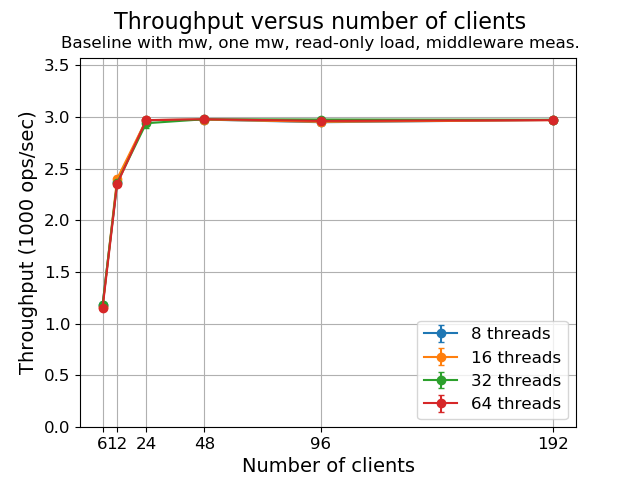
\includegraphics[width=1.0\linewidth,trim={0px 0px 0px 0px},clip]{img/plot/mwb1-ro-tp_mw.png}
  \caption{Read-only throughput}
  \label{fig:mwb1-ro-tp_mw}
\end{subfigure}%
\begin{subfigure}{.5\textwidth}
  \centering
  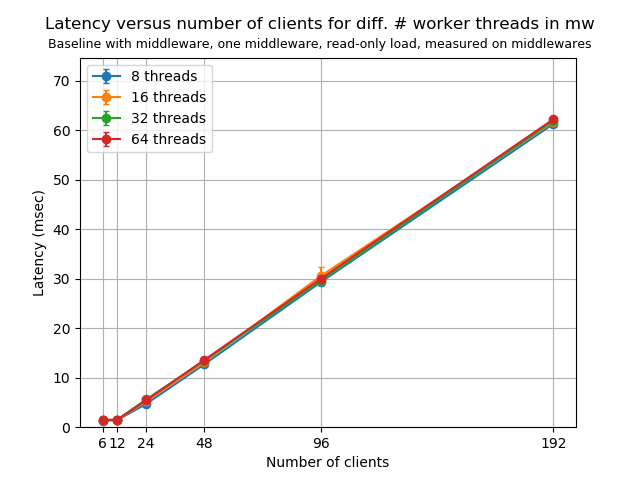
\includegraphics[width=1.0\linewidth,trim={0px 0px 0px 0px},clip]{img/plot/mwb1-ro-lat_mw.png}
  \caption{Read-only latency}
  \label{fig:mwb1-ro-lat_mw}
\end{subfigure}
\caption{Throughput and latency values for the read-only workload for baseline with middleware experiment with one middleware.}
\label{fig:mwb1-ro_mw}
\end{figure}

\begin{figure}[h]
\centering
\begin{subfigure}{.33\textwidth}
  \centering
  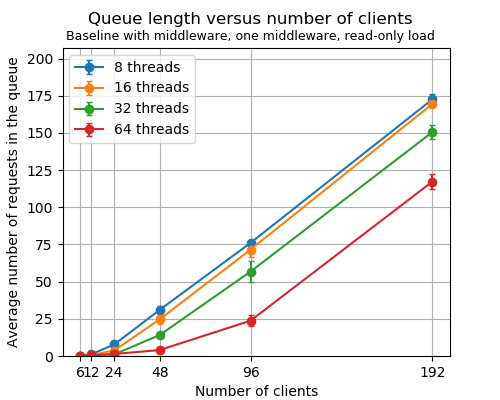
\includegraphics[width=1.0\linewidth,trim={0px 0px 0px 0px},clip]{img/plot/mwb1-ro-qlen-mini.png}
  \caption{Avg. queue length}
  \label{fig:mwb1-ro-qlen-mini}
\end{subfigure}%
\begin{subfigure}{.33\textwidth}
  \centering
  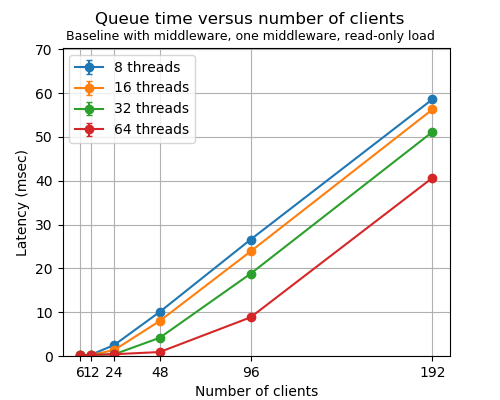
\includegraphics[width=1.0\linewidth,trim={0px 0px 0px 0px},clip]{img/plot/mwb1-ro-qtime-mini.png}
  \caption{Avg. queue time}
  \label{fig:mwb1-ro-qtime-mini}
\end{subfigure}%
\begin{subfigure}{.33\textwidth}
  \centering
  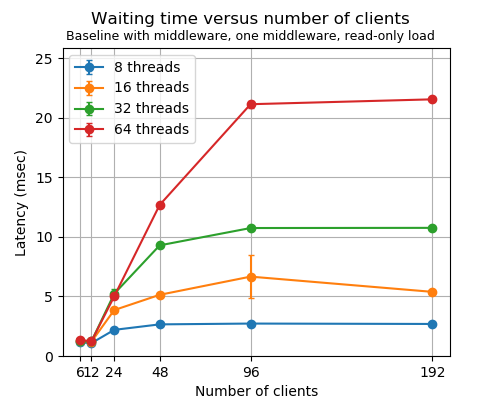
\includegraphics[width=1.0\linewidth,trim={0px 0px 0px 0px},clip]{img/plot/mwb1-ro-wtime-mini.png}
  \caption{Avg. waiting time}
  \label{fig:mwb1-ro-wtime-mini}
\end{subfigure}
\caption{Average queue lengths, queue times and waiting times for the read-only workload for baseline with middleware experiment with one middleware.}
\label{fig:mwb1-ro-mini}
\end{figure}

\begin{figure}[h]
\centering
\begin{subfigure}{.5\textwidth}
  \centering
  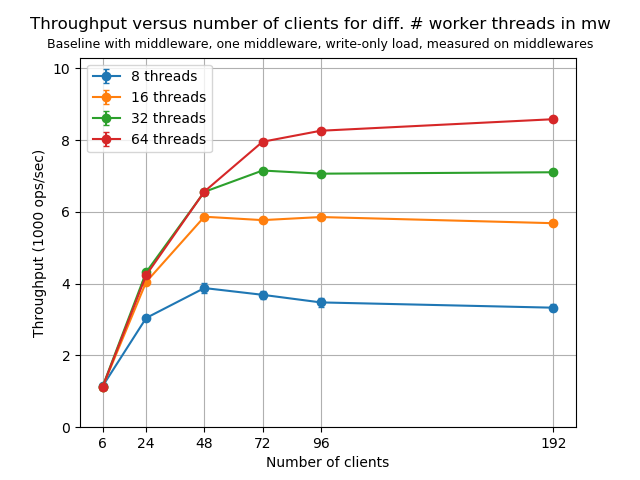
\includegraphics[width=1.0\linewidth,trim={0px 0px 0px 0px},clip]{img/plot/mwb1-wo-tp_mw.png}
  \caption{Write-only throughput}
  \label{fig:mwb1-wo-tp_mw}
\end{subfigure}%
\begin{subfigure}{.5\textwidth}
  \centering
  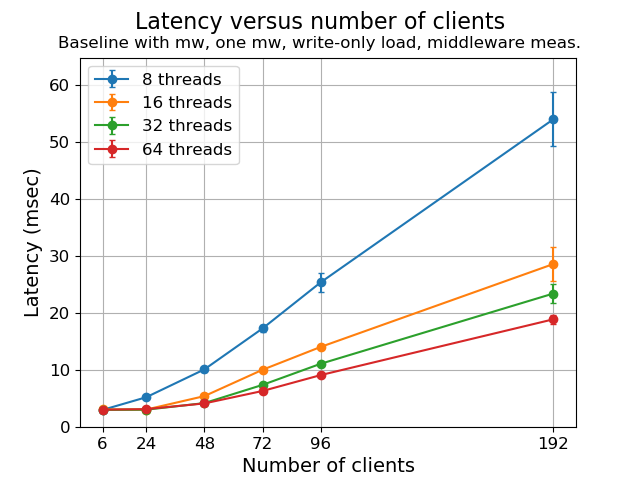
\includegraphics[width=1.0\linewidth,trim={0px 0px 0px 0px},clip]{img/plot/mwb1-wo-lat_mw.png}
  \caption{Write-only latency}
  \label{fig:mwb1-wo-lat_mw}
\end{subfigure}
\caption{Throughput and latency values for the write-only workload for baseline with middleware experiment with one middleware.}
\label{fig:mwb1-wo_mw}
\end{figure}

\begin{figure}[h]
\centering
\begin{subfigure}{.33\textwidth}
  \centering
  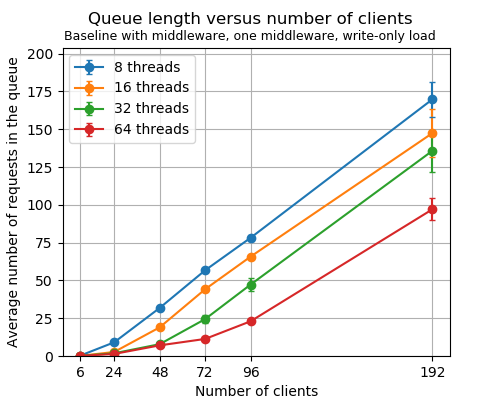
\includegraphics[width=1.0\linewidth,trim={0px 0px 0px 0px},clip]{img/plot/mwb1-wo-qlen-mini.png}
  \caption{Avg. queue length}
  \label{fig:mwb1-wo-qlen-mini}
\end{subfigure}%
\begin{subfigure}{.33\textwidth}
  \centering
  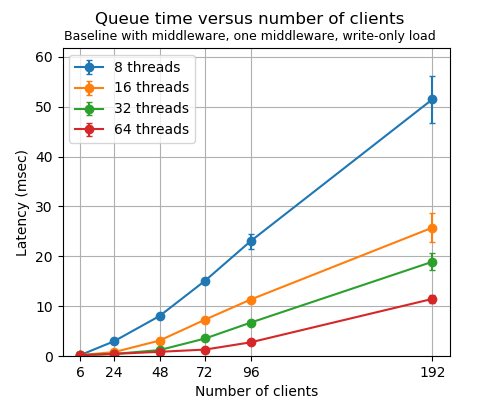
\includegraphics[width=1.0\linewidth,trim={0px 0px 0px 0px},clip]{img/plot/mwb1-wo-qtime-mini.png}
  \caption{Avg. queue time}
  \label{fig:mwb1-wo-qtime-mini}
\end{subfigure}%
\begin{subfigure}{.33\textwidth}
  \centering
  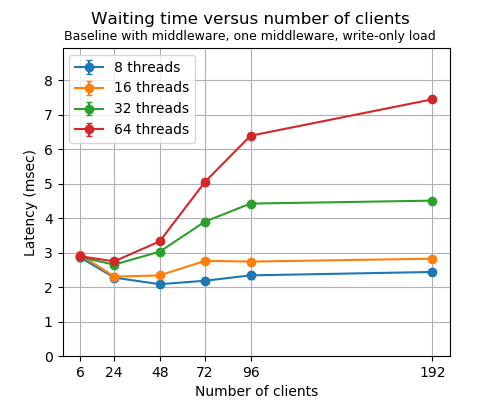
\includegraphics[width=1.0\linewidth,trim={0px 0px 0px 0px},clip]{img/plot/mwb1-wo-wtime-mini.png}
  \caption{Avg. waiting time}
  \label{fig:mwb1-wo-wtime-mini}
\end{subfigure}
\caption{Average queue lengths, queue times and waiting times for the write-only workload for baseline with middleware experiment with one middleware.}
\label{fig:mwb1-wo-mini}
\end{figure}

\subsubsection{Explanation} \label{sec:mwb1-exp}
Plots in Figures \ref{fig:mwb1-ro_mw} and \ref{fig:mwb1-wo_mw} illustrate the throughput and response time measured on the middleware, respectively for read-only and write-only loads. With the read-only load, we observe a trend quite similar to the read-only results in baselines without middleware. Until we reach around 24 clients we can observe quite an increase in the throughput which is only accompanied by relatively smaller increases in the response time, regardless of the size of the thread pool in middleware. Afterwards, the trend is again the same for different number of threads: an increase in the number of clients results in a linear increase in the response times and does not change the average throughput obtained. Therefore, we state that the system saturates when there are around 24 clients in the system, regardless of the size of the worker thread pool in the middleware.
\par The reason behind this saturation is familiar to us from the previous sections: server to middleware connection is limited by a bandwidth of 12MB per second, so the server cannot send more replies because of the network limitations. This saturation happens so early in the system that we do not get to observe the effects of different threads in middleware. In other words, the middleware works efficiently even with 8 worker threads until the system saturates, so any number of worker threads could hypothetically handle more work if the server could be able respond more clients. It should also be noted that we cannot observe any network-wise limitations on top of the server-side send bottleneck and the CPU usage is fairly low for all the machines in the system ($80\%$ idle time at worst), as per dstat and iperf. \change{marginal change for tmw's}
\par \change{this whole paragraph needs review} Figure \ref{fig:mwb1-ro-qlen-mini} illustrates the average queue lengths for various configurations. As the system is network bound for this workload, the server can only reply a portion of the requests while the other thread wait to send their requests. We expect these number of waiting threads to be very small, if the number of clients are smaller than the number of middleware threads. For the range the number of clients are greater than the worker of threads every additional client should increase the average queue length linearly. The plot confirms both our intuitions as for every different number of worker threads the queue length stay close to zero until the number of clients exceed the number of worker threads and the difference in queue lengths for the linear region is proportional to the number of clients. Lastly, we can see by comparing the values in Figures \ref{fig:mwb1-ro-qlen-mini} and \ref{fig:mwb1-ro-qtime-mini} that the queue times and the queue lengths have an approximately linear correlation as expected. The reason behind such relation is that as the system is network bound it is not the middleware but the server side that affects the queue times in the saturated region so changing the number of worker threads does not make a difference.
\\
\par In the write-only case, we can observe a trend which is completely different from the read-only case, as the network is no longer our bottleneck. The trend until reaching 24 clients is similar with the read-only case as differences in the number of worker threads do not correspond to a difference in terms of the performance of the system, except 8 thread configuration which saturates around 24 clients. This is because the system is under-saturated for 16, 32 and 64 threads so we can expect their throughput and response time statistics to go hand in hand as the number of worker threads do not result in a noticeable difference in these metrics under light workload conditions. As we introduce more and more clients to the system we observe more divergence with respect to performance for different number of threads in the middleware.
\par We can see that there are saturation points with different values in both axes for different worker thread configurations. Due to the inherent limitations of the experiment, the number of clients were not explored in depth for us to pinpoint exact saturation points for all worker thread configurations. For example, we say that 96 clients is where the 64 thread setup saturates, but we believe a comparably fine-grained study might show that the system saturates with fewer number of clients than 96.
\par This time, the comparison of queue lengths and queue times (Figures \ref{fig:mwb1-wo-qlen-mini} and \ref{fig:mwb1-wo-qtime-mini}, respectively) yield a different interpretation. We can clearly see that, for the same queue lengths, different number of worker threads result in different scaling factors for the queue times. Moreover, queue length to queue time ratio increases with the number of worker threads. What that means is that the systems could process a longer queue for the same queueing times in average, since there will be more worker threads available to handle the requests.
\par After interpreting all the relevant plots we can conclude that for the write-only workload the middleware is the bottleneck. dstat measurements are also cross-checked and we do not report any network or CPU usage limit for the write-only configurations. We say that the number of worker threads is the limiting parameter for our experiments for the write-only load and more worker threads mean better system performances. As a manifestation of this interpretation, we could see that we cannot achieve the levels of throughput reached in the first part of the baseline without middleware, as the middleware introduces a considerable amount of overhead between the clients and the server.
\par However, we cannot assert the system performance would continuously increase as we introduce more and more worker threads into the middleware. Looking at the Figures \ref{fig:mwb1-ro-wtime-mini} and \ref{fig:mwb1-wo-wtime-mini} we can see that waiting times (server service times) and the number of working thread in the middleware are inversely proportional and we can expect the waiting times (server service times) to increase more as we keep increasing the worker threads. For our experimental setup this is an expected result as we configure our servers to only use one thread. \change{BE WARY, rethink that, compare against csb values}

\subsection{Two Middlewares} \label{sec:mwb2}
Second experiment for this section again has an environment with three clients and one server, but two middlewares instead of one. Again, we vary the workloads, number of clients and number of worker threads in the middleware and discuss the results.

\begin{figure}[h]
\centering
\begin{subfigure}{.5\textwidth}
  \centering
  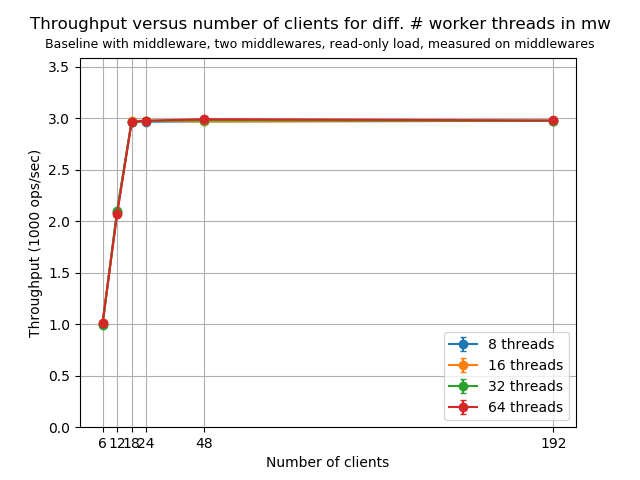
\includegraphics[width=1.0\linewidth,trim={0px 0px 0px 0px},clip]{img/plot/mwb2-ro-tp_mw.png}
  \caption{Read-only throughput}
  \label{fig:mwb2-ro-tp_mw}
\end{subfigure}%
\begin{subfigure}{.5\textwidth}
  \centering
  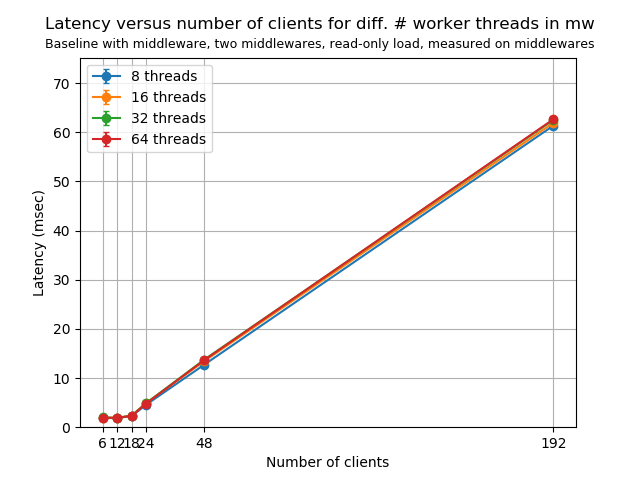
\includegraphics[width=1.0\linewidth,trim={0px 0px 0px 0px},clip]{img/plot/mwb2-ro-lat_mw}
  \caption{Read-only latency}
  \label{fig:mwb2-ro-lat_mw}
\end{subfigure}
\caption{Throughput and latency values for the read-only workload for baseline with middleware experiment with two middlewares.}
\label{fig:mwb2-ro_mw}
\end{figure}

\begin{figure}[h]
\centering
\begin{subfigure}{.33\textwidth}
  \centering
  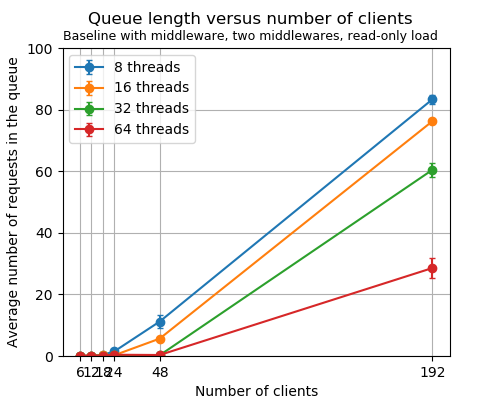
\includegraphics[width=1.0\linewidth,trim={0px 0px 0px 0px},clip]{img/plot/mwb2-ro-qlen-mini.png}
  \caption{Avg. queue length}
  \label{fig:mwb2-ro-qlen-mini}
\end{subfigure}%
\begin{subfigure}{.33\textwidth}
  \centering
  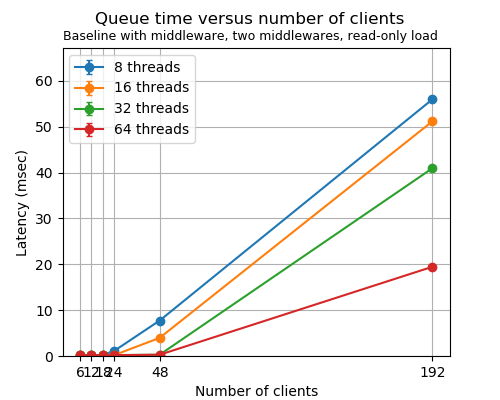
\includegraphics[width=1.0\linewidth,trim={0px 0px 0px 0px},clip]{img/plot/mwb2-ro-qtime-mini.png}
  \caption{Avg. queue time}
  \label{fig:mwb2-ro-qtime-mini}
\end{subfigure}%
\begin{subfigure}{.33\textwidth}
  \centering
  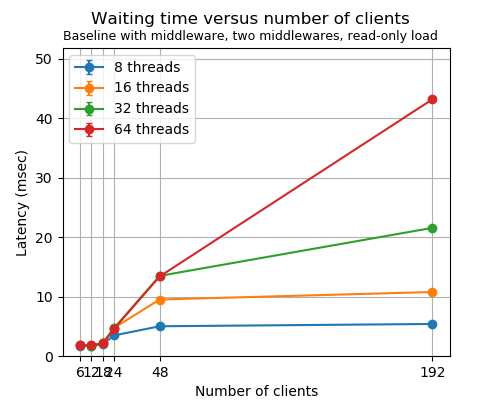
\includegraphics[width=1.0\linewidth,trim={0px 0px 0px 0px},clip]{img/plot/mwb2-ro-wtime-mini.png}
  \caption{Avg. waiting time}
  \label{fig:mwb2-ro-wtime-mini}
\end{subfigure}
\caption{Average queue lengths, queue times and waiting times (server service times) for the read-only workload for baseline with middleware experiment with two middlewares.}
\label{fig:mwb2-ro-mini}
\end{figure}

\begin{figure}[h]
\centering
\begin{subfigure}{.5\textwidth}
  \centering
  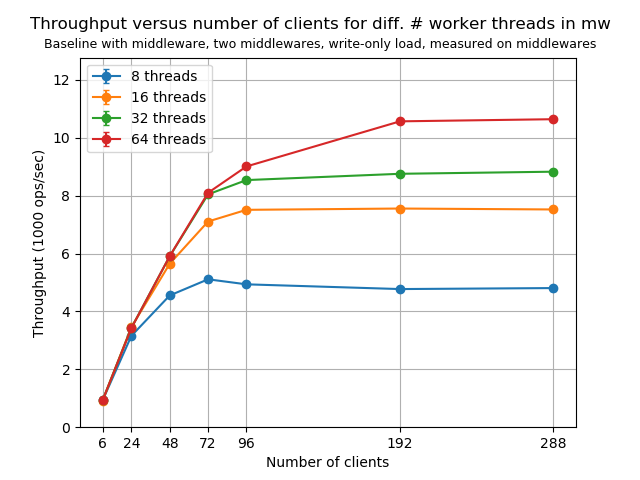
\includegraphics[width=1.0\linewidth,trim={0px 0px 0px 0px},clip]{img/plot/mwb2-wo-tp_mw.png}
  \caption{Write-only throughput}
  \label{fig:mwb2-wo-tp_mw}
\end{subfigure}%
\begin{subfigure}{.5\textwidth}
  \centering
  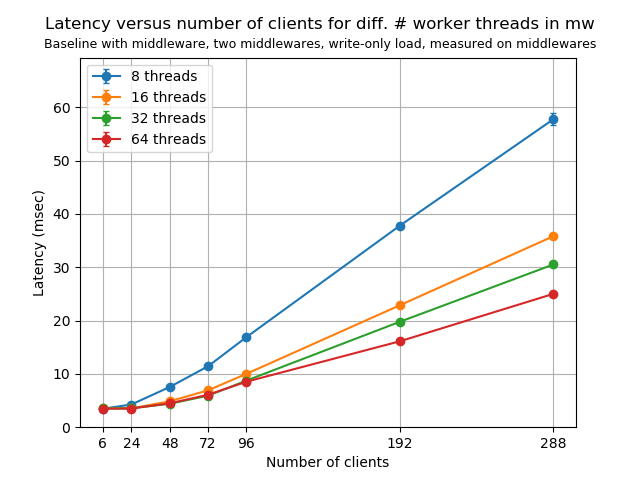
\includegraphics[width=1.0\linewidth,trim={0px 0px 0px 0px},clip]{img/plot/mwb2-wo-lat_mw}
  \caption{Write-only latency}
  \label{fig:mwb2-wo-lat_mw}
\end{subfigure}
\caption{Throughput and latency values for the write-only workload for baseline with middleware experiment with two middlewares.}
\label{fig:mwb2-wo_mw}
\end{figure}

\begin{figure}[h]
\centering
\begin{subfigure}{.33\textwidth}
  \centering
  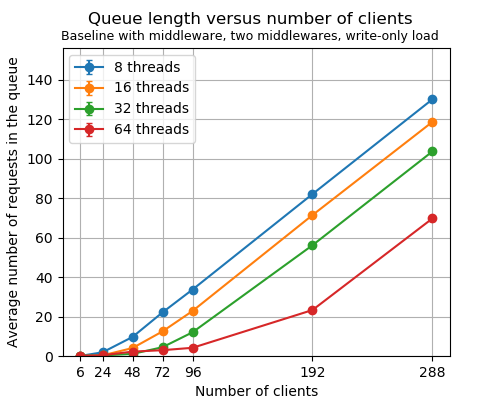
\includegraphics[width=1.0\linewidth,trim={0px 0px 0px 0px},clip]{img/plot/mwb2-wo-qlen-mini.png}
  \caption{Avg. queue length}
  \label{fig:mwb2-wo-qlen-mini}
\end{subfigure}%
\begin{subfigure}{.33\textwidth}
  \centering
  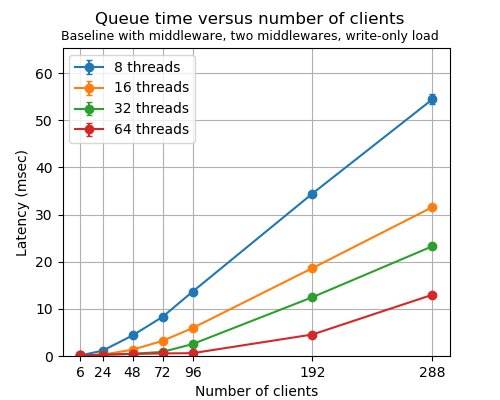
\includegraphics[width=1.0\linewidth,trim={0px 0px 0px 0px},clip]{img/plot/mwb2-wo-qtime-mini.png}
  \caption{Avg. queue time}
  \label{fig:mwb2-wo-qtime-mini}
\end{subfigure}%
\begin{subfigure}{.33\textwidth}
  \centering
  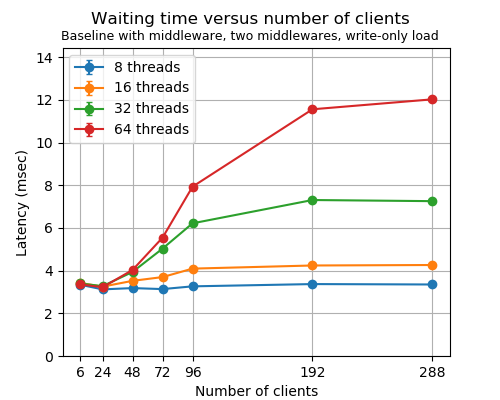
\includegraphics[width=1.0\linewidth,trim={0px 0px 0px 0px},clip]{img/plot/mwb2-wo-wtime-mini.png}
  \caption{Avg. waiting time (server service times)}
  \label{fig:mwb2-wo-wtime-mini}
\end{subfigure}
\caption{Average queue lengths, queue times and waiting times (server service times) for the write-only workload for baseline with middleware experiment with two middlewares.}
\label{fig:mwb2-wo-mini}
\end{figure}

\subsubsection{Explanation} \label{sec:mwb2-exp}
Plots in Figures \ref{fig:mwb2-wo_mw} and \ref{fig:mwb2-wo-mini} illustrate various statistics for the write-only load. We see results similar to the one middleware setup. System saturates at different number of clients for different number of worker threads. For the same average queue lengths, the queue times shorten as the number of worker threads increases. Again the number of working threads is our limiting factor for the system performance. Thus, we conclude the middleware being the bottleneck for the write-only case with two middlewares. Again, we find it intuitive that the statistics for the one middleware setup matches those of the two middleware setup with the half amount of worker threads, as it was the case with the read-only workload.
\par An intuitive correlation is as follows: statistics for the 8, 16 and 32 thread configurations for two middleware setup matches respectively with the 16, 32 and 64 thread settings for the one middleware. In other words, doubling the number of threads for one midleware has the same effects as introducing another middleware with the same number of threads on the system. Although, we can only say that for our experimental setup and configurations and this equivalence may not hold for factors much greater than two.
\par Results for the read-only workload is almost exactly the same as those from the setting with one middleware, as the bottleneck of the system is stays the same, which was detailed in the previous sections. Both the throughput and latency values (Figure \ref{fig:mwb2-ro_mw}) with respect to number of clients is quite similar to those of the configuration with one server, stemming from the same limitations.
\par Figure \ref{fig:mwb2-ro-mini} illustrates the average queue length, queue time and waiting time (server service times) statistics for this experiment on read-only load. Here, we warn the reader to be careful when comparing the queue lengths for two and one middleware setups directly as the reported queue length is averaged over the middlewares. That is, to approximate the total number of requests waiting in the middleware queues one should multiply the averaged value by the number of middlewares in the environment. Lastly, we note the relation between queue lengths and queue times is the same as in the one middleware setup.\change{waiting times}

\subsection{Summary} \label{sec:mwb-summary}
Tables \ref{tab:mwb1-summary} and \ref{tab:mwb2-summary} reports the results for the middleware experiments, respectively the one middleware and the two middleware setups. All of the results shown in the tables are from the 64 worker thread configuration of the respective experiments.
\\
\par First thing we can do is to compare the values aggregated by the clients with those obtained by the middlewares. Throughput and miss rate statistics show that they are approximately, but not absolutely, equal. As we aggregate data after cutting the warm-up and cool-down periods on both client and middleware outputs, this is a natural result. It is verified through additional experiments that the statistics match completely if the aggregations were to be done on the entirety of the data collected by both sides.
\par For response times, there is a significant but consistent difference between the averaged values reported by the middlewares and the clients. Client response times also include the time a request requires to travel from a client to a middleware and its reply from the middleware to the client, similarly. The difference between the aforementioned response times are equal to the round-trip time (RTT) of the clients and serves for the respective experiments. We can also observe that this RTT is not always constant. It is again natural as the network characteristics may fluctuate in between (and even during) experiments and we also employ multiple clients on different physical machines, we expect not a constant difference but a RTT that samples a probability distribution.
\par As discussed in Section \ref{sec:ov-methodology}, we populate the server with the 99\% of the keys we will use in the read-only experiments. This, in turn, (together with the fact that we do not allow any expiry) means that for each read-only experiment we should observe a miss rate around 1\% when looked from both middleware and client perspectives. Looking at the reported miss rates we can see that the values observed is in line with our expectations and client results corroborate the middleware aggregations.
\\
\par As explained in the preceding sections, maximum read-only throughput is just under 3000 requests per second, for both experiments. As the system is network bound under read-only load, changes in the number of middleware and the number of worker threads per middleware change neither where the system saturates, nor the maximum throughput achieved. Write-only experiments present us with a different picture. As the bottleneck of the system is middleware for both configurations, we see an increase in the maximum throughput obtained when we add a new middleware to the environment. This holds true not only for the 64 thread configuration which gives the best performance but for all sizes of the worker-thread pool. Looking once again at the Figures \ref{fig:mwb1-wo_mw} and \ref{fig:mwb2-wo_mw} we can see the saturation points for all worker-thread configurations go up with respect to clients. To illustrate, one middleware with 16 worker threads is already saturated with 48 clients but with two middlewares of 16 threads we see a continuous increase lasting between 72 and 96 clients. As discussed before, doubling the the number of middlewares has approximately the same effects on the system performance as doubling the size of the worker-thread pools in middlewares.
\par Lastly, we note that even with two middlewares of 64 threads we cannot reach the maximum throughput achieved without middleware in the environment. We say the parameter values explored through experiments of this section is not enough to obtain performances comparable to the ones in Section \ref{sec:csb1}. For the same number of clients, additional network delays incurred and the overhead of the middlewares result in lower performances with the systems with middlewares.
\change{I should talk about queueing times and response times here possibly}

\begin{table}[h]
\centering
{Maximum throughput for one middleware.}
\begin{tabular}{|l|p{2.3cm}|p{2.3cm}|p{2.7cm}|p{2.3cm}|}
\hline                       & Throughput        & {\small Response time}      & {\small Avg. queue time} & Miss rate \\ 
\hline Reads: Meas. on mw       & $2969.3 \pm 1.5$  & $5.413 \pm 0.021$  & $0.406 \pm 0.011$  & $0.0095404$ \\ 
\hline Reads: Meas. on clients  & $2969.3 \pm 1.8$  & $8.083 \pm 0.004$  & n/a                & $0.0095287$ \\ 
\hline Writes: Meas. on mw      & $8264.1 \pm 17.5$ & $9.125 \pm 0.017$  & $2.740 \pm 0.015$  & n/a \\ 
\hline Writes: Meas. on clients & $8263.5 \pm 17.3$ & $11.628 \pm 0.026$ & n/a                & n/a \\ 
\hline 
\end{tabular}
\caption{Summary of the baseline with one middleware.} \label{tab:mwb1-summary}
\end{table}

\begin{table}[h]
\centering
{Maximum throughput for two middlewares.}
\begin{tabular}{|l|p{2.3cm}|p{2.3cm}|p{2.7cm}|p{2.3cm}|}
\hline                      & Throughput         & {\small Response time}      & {\small Avg. queue time} & Miss rate \\ 
\hline Reads: Meas. on mw       & $2964.3 \pm 0.3$   & $2.288 \pm 0.061$  & $0.181 \pm 0.001$  & $0.0093647$ \\ 
\hline Reads: Meas. on clients  & $2964.4 \pm 0.8$   & $6.077 \pm 0.002$  & n/a                & $0.0095260$ \\ 
\hline Writes: Meas. on mw      & $10566.1 \pm 59.6$ & $16.121 \pm 0.118$ & $4.557 \pm 0.039$  & n/a     \\ 
\hline Writes: Meas. on clients & $10566.4 \pm 59.6$ & $18.206 \pm 0.105$ & n/a                & n/a     \\ 
\hline 
\end{tabular}
\caption{Summary of the baseline with two middlewares.} \label{tab:mwb2-summary}
\end{table}

\section{Throughput for Writes} \label{sec:tpfw}
This section inspects the system with three clients, two middlewares and three servers, under write-only load. Number of worker-threads and the number of clients are varied in order to understand the characteristic of the system through different configurations.

\subsection{Full System} \label{sec:tpfw-fs}
\begin{figure}[h]
\centering
\begin{subfigure}{.5\textwidth}
  \centering
  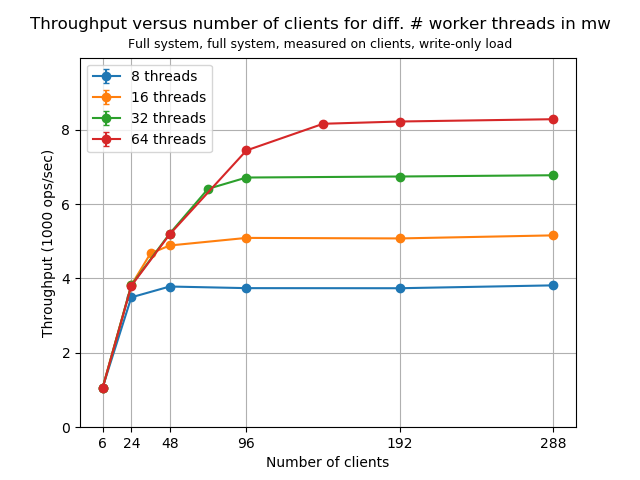
\includegraphics[width=1.0\linewidth,trim={0px 0px 0px 0px},clip]{img/plot/tpfw-tp_mw.png}
  \caption{Throughput}
  \label{fig:tpfw-tp_mw}
\end{subfigure}%
\begin{subfigure}{.5\textwidth}
  \centering
  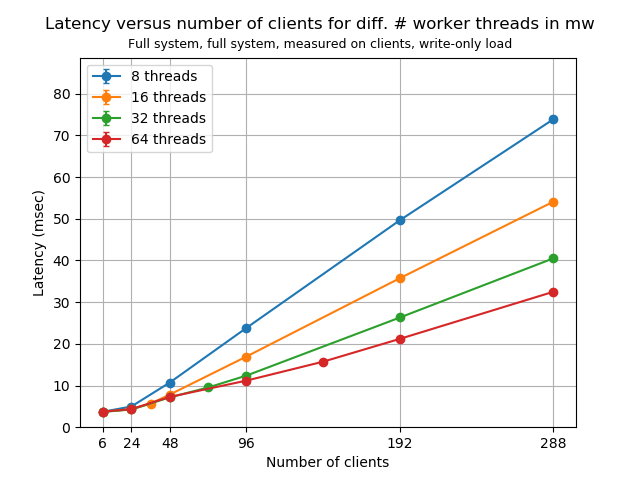
\includegraphics[width=1.0\linewidth,trim={0px 0px 0px 0px},clip]{img/plot/tpfw-lat_mw.png}
  \caption{Latency}
  \label{fig:tpfw-lat_mw}
\end{subfigure}
\caption{Throughput and latency values for the throughput for writes experiment, write-only workload.}
\label{fig:tpfw_mw}
\end{figure}

Figures \ref{fig:tpfw-tp_mw} and \ref{fig:tpfw-lat_mw} illustrate the average throughputs and response times of the system under different configurations. Each line represents a setup with a different number of threads for both plots. Results are similar to those analysed in Section \ref{sec:mwb2}, as the setup stays the same except the increase in the number of servers the system has. We see each configuration saturates at different points, since the middleware is the bottleneck of the system. Each of them conforms to the same trend: throughput gains become minimal and response times start to form a linear pattern as we move closer to the number of clients which saturates a given configuration. 
\begin{figure}[h]
\centering
\begin{subfigure}{.33\textwidth}
  \centering
  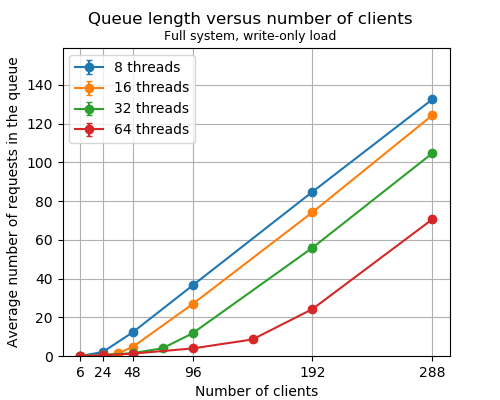
\includegraphics[width=1.0\linewidth,trim={0px 0px 0px 0px},clip]{img/plot/tpfw-qlen_mw.png}
  \caption{Avg. queue length}
  \label{fig:tpfw-qlen_mw}
\end{subfigure}%
\begin{subfigure}{.33\textwidth}
  \centering
  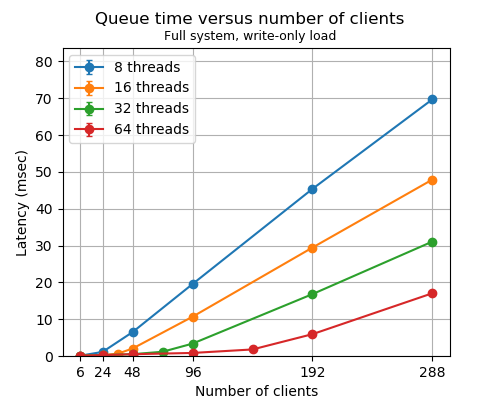
\includegraphics[width=1.0\linewidth,trim={0px 0px 0px 0px},clip]{img/plot/tpfw-qtime_mw.png}
  \caption{Avg. queue time}
  \label{fig:tpfw-qtime_mw}
\end{subfigure}%
\begin{subfigure}{.33\textwidth}
  \centering
  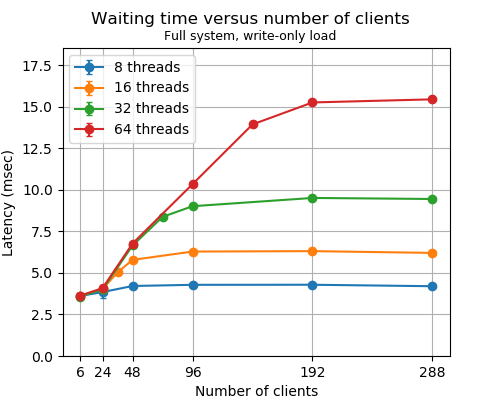
\includegraphics[width=1.0\linewidth,trim={0px 0px 0px 0px},clip]{img/plot/tpfw-wtime_mw.png}
  \caption{Avg. waiting time (server service times)}
  \label{fig:tpfw-wtime_mw}
\end{subfigure}
\caption{Average queue lengths, queue times and waiting times (server service times) for the throughput for writes experiment, write-only workload.}
\label{fig:tpfw_stats_mw}
\end{figure}
\par For 8, 16, 32 and 64 worker-threads we state the saturation points are around 24, 36, 72 and 144 clients. With the exception of the 8 thread setup, we can see that the number of clients a saturated system can handle doubles as we double the worker-threads in the middleware. It is in line with our expectations as this ratio of number of worker-threads to the number of clients at the point of saturation should hold true for different number of worker threads with same configuration. Since middlewares are the bottlenecks of this setup, we except there should be enough requests in the systems waiting to be handled. This, in turn, means an increase in the number of worker-threads should amount to an approximately linear increase in the average number of requests that can be handled for a given period, which is indeed corroborated by the aforementioned results. Reader should note that the 8 worker thread setting has not the same level of granularity as the other settings and experiences a much sharper increase before leveling off. This points to the need for a finer grained search in the 6-24 client range, as the saturation of the 8 thread configuration is believed to be expected earlier than 24 clients, much likely around 18 clients considering the pattern described above.
\par Figures \ref{fig:tpfw-qlen_mw} and \ref{fig:tpfw-qtime_mw} respectively illustrate the average queue length and queueing time statistics for the throughput for writes experiment. As the experimental setup of this section is quite similar to the one in baseline experiments with two middlewares in Section \ref{sec:mwb2}, it is of no surprise that we obtain similar trends related to request queue. We can verify the saturation points for the different thread configurations as the points where lines in both plots become completely linear. We can again observe that corresponding lines in queue length and queue time plots have different slopes. For the system to reach a chosen queue length, we would need more clients with configurations with more threads. What that indicates is an increase in the number of threads in the middleware increases performance by reducing the queueing times, so the number of middleware threads is our limiting factor for this experiment.
\change{waiting times}

\subsubsection{Explanation} \label{sec:tpfw-exp}
\begin{figure}[h]
\centering
\begin{subfigure}{.5\textwidth}
  \centering
  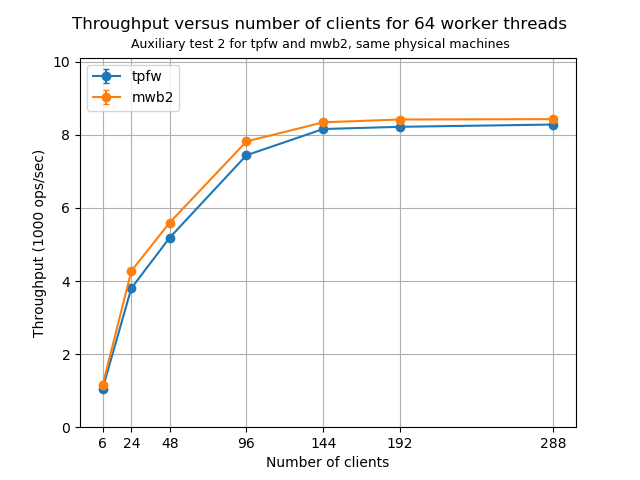
\includegraphics[width=1.0\linewidth,trim={0px 0px 0px 0px},clip]{img/plot/auxiliary-2-tp_mw.png}
  \caption{Throughput}
  \label{fig:auxiliary-2-tp_mw}
\end{subfigure}%
\begin{subfigure}{.5\textwidth}
  \centering
  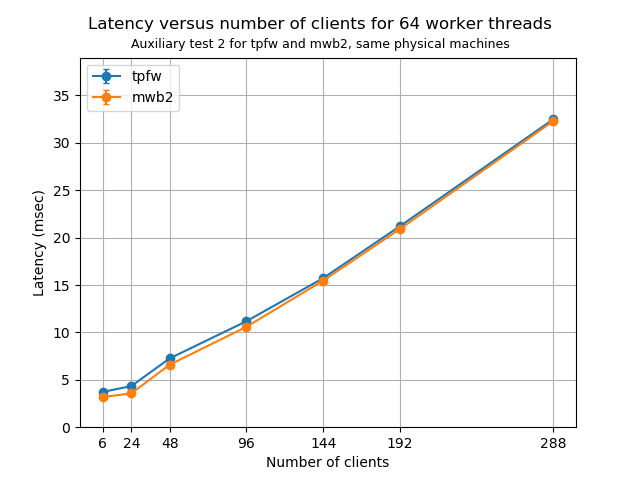
\includegraphics[width=1.0\linewidth,trim={0px 0px 0px 0px},clip]{img/plot/auxiliary-2-lat_mw.png}
  \caption{Latency}
  \label{fig:auxiliary-2-lat_mw}
\end{subfigure}
\caption{Throughput and latency values for an auxiliary experiment, write-only workload with 64 worker threads on middlewares. tpfw stands for the throughput for writes experiment, whereas the mwb2 denotes the middleware baseline experiment with two baselines.}
\label{fig:auxiliary-2_mw}
\end{figure}

\subsection{Summary} \label{sec:tpfw-summary}
\change{see how the predicted values do not really match the acutal values}
\begin{table}[h]
\small
\centering
{Maximum throughput for the full system}
\begin{tabular}{|p{5.1cm}|p{2.1cm}|p{1.9cm}|p{1.9cm}|p{1.9cm}|}
\hline                                            & WT=8               & WT=16             & WT=32             & WT=64             \\ 
\hline Throughput (Middleware)                    & $3492.9 \pm 49.1$  & $4673.6 \pm 23.5$ & $6411.0 \pm 5.0$  & $8161.1 \pm 24.9$  \\ 
\hline Throughput (Derived from MW response time) & $3459.6 \pm 205.4$ & $4698.3 \pm 40.1$ & $6246.1 \pm 5.8$  & $8124.1 \pm 27.3$ \\ 
\hline Throughput (Client)                        & $3492.8 \pm 49.1$  & $4674.3 \pm 23.4$ & $6412.2 \pm 6.2$  & $8161.5 \pm 25.2$ \\ 
\hline Average time in queue                      & $1.112 \pm 0.062$  & $0.622 \pm 0.006$ & $1.148 \pm 0.010$ & $1.779 \pm 0.017$ \\ 
\hline Average length of queue                    & $2.0 \pm 0.0$      & $1.4 \pm 0.1$     & $4.0 \pm 0.2$     & $8.6 \pm 1.2$     \\ 
\hline Average time waiting for memcached         & $3.9 \pm 0.4$      & $5.0 \pm 0.1$     & $8.4 \pm 0.0$     & $13.9 \pm 0.0$    \\ 
\hline 
\end{tabular}
\caption{Summary of the throughput for writes experiments.} \label{tab:tpfw-summary}
\end{table}

\section{Gets and Multi-gets} \label{sec:gmg}
\begin{figure}[h]
\begin{subfigure}{.5\textwidth}
  \centering
  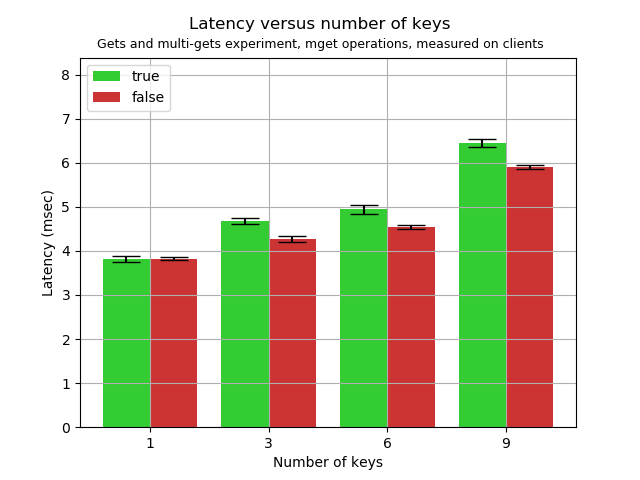
\includegraphics[width=1.0\linewidth ,trim={0 0 0 0},clip]{img/plot/gmg-mget-lat_cli.png}
  \caption{Latency}
  \label{fig:gmg-mget-lat_cli}
\end{subfigure}%
\begin{subfigure}{.5\textwidth}
  \centering
  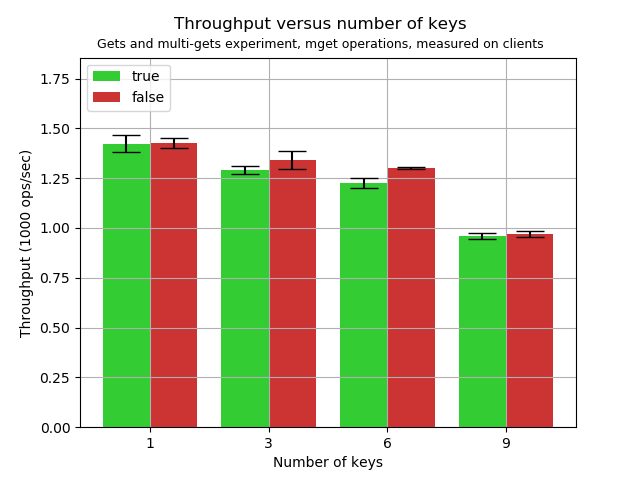
\includegraphics[width=1.0\linewidth ,trim={0 0 0 0},clip]{img/plot/gmg-mget-tpt_cli.png}
  \caption{Throughput}
  \label{fig:gmg-mget-tpt_cli}
\end{subfigure}
\caption{Throughput and response times of sharded and non-sharded reads in different key size experiments}
\label{fig:gmg-mget_cli}
\end{figure}

\subsection{Sharded Case} \label{sec:gmg-true}
\begin{figure}[h]
\begin{subfigure}{.5\textwidth}
  \centering
  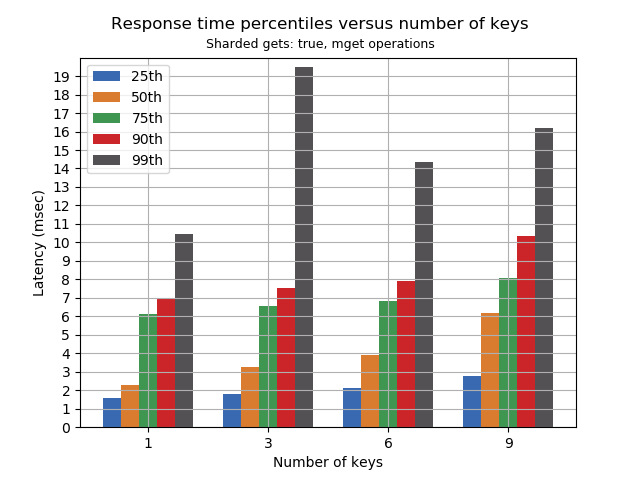
\includegraphics[width=1.0\linewidth ,trim={0 0 0 0},clip]{img/plot/gmg-perc-true.png}
  \caption{Sharded case}
  \label{fig:gmg-perc-true}
\end{subfigure}%
\begin{subfigure}{.5\textwidth}
  \centering
  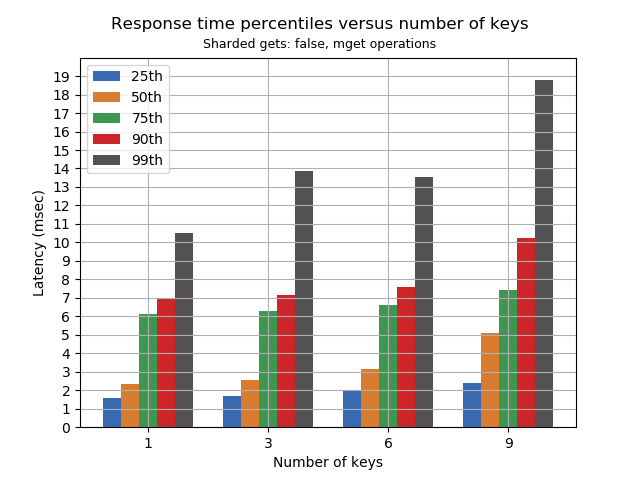
\includegraphics[width=1.0\linewidth ,trim={0 0 0 0},clip]{img/plot/gmg-perc-false.png}
  \caption{Non-sharded case}
  \label{fig:gmg-perc-false}
\end{subfigure}
\caption{25th, 50th, 75th, 90th and 99th percentiles of sharded and non-sharded reads, for 1, 3, 6 and 9 key cases. Instead of their respective sections each, plots are provided side by side together to help the reader when comparing two cases.}
\label{fig:gmg-perc}
\end{figure}

\subsubsection{Explanation} \label{sec:gmg-true-exp}

\subsection{Non-sharded Case} \label{sec:gmg-false}

\subsubsection{Explanation} \label{sec:gmg-false-exp}

\subsection{Histogram} \label{sec:gmg-hist}
\begin{figure}[h]
\begin{subfigure}{.5\textwidth}
  \centering
  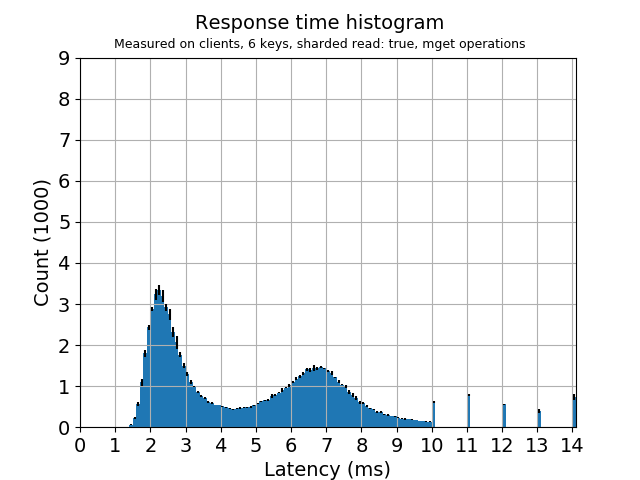
\includegraphics[width=1.0\linewidth ,trim={0 0 0 0},clip]{img/plot/gmg-hist6-true-mget_clients.png}
  \caption{Sharded case, client measurements}
  \label{fig:gmg-hist6-true-mget_clients}
\end{subfigure}%
\begin{subfigure}{.5\textwidth}
  \centering
  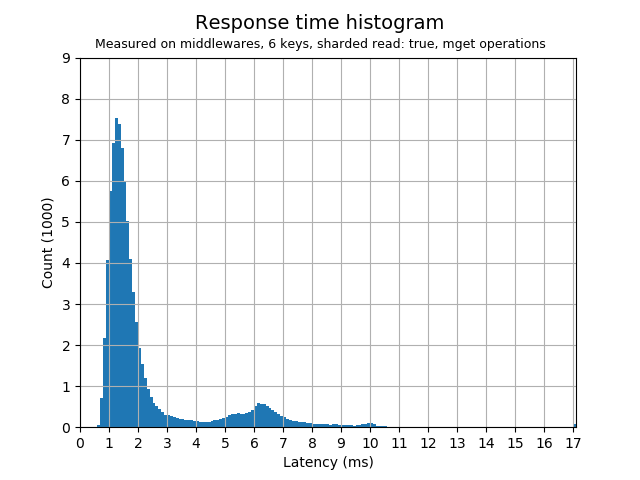
\includegraphics[width=1.0\linewidth ,trim={0 0 0 0},clip]{img/plot/gmg-hist6-true-mget_middlewares.png}
  \caption{Sharded case, middleware measurements}
  \label{fig:gmg-hist6-true-mget_middlewares}
\end{subfigure}
\begin{subfigure}{.5\textwidth}
  \centering
  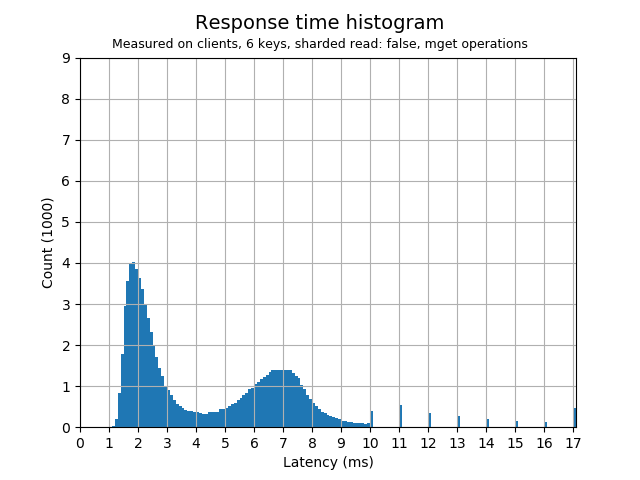
\includegraphics[width=1.0\linewidth ,trim={0 0 0 0},clip]{img/plot/gmg-hist6-false-mget_clients.png}
  \caption{Non-sharded case, client measurements}
  \label{fig:gmg-hist6-false-mget_clients}
\end{subfigure}%
\begin{subfigure}{.5\textwidth}
  \centering
  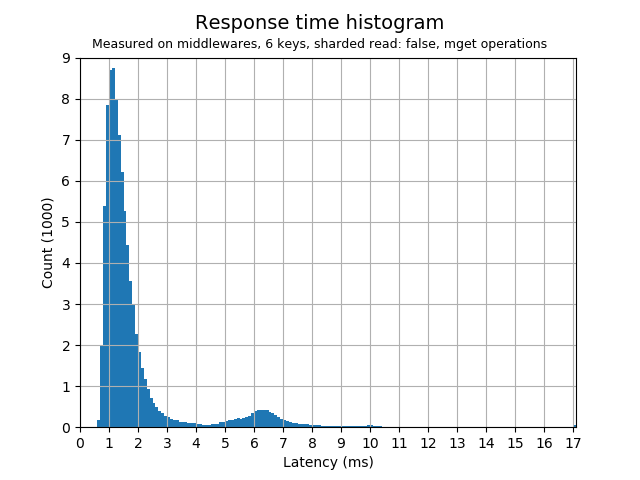
\includegraphics[width=1.0\linewidth ,trim={0 0 0 0},clip]{img/plot/gmg-hist6-false-mget_middlewares.png}
  \caption{Non-sharded case, middleware measurements}
  \label{fig:gmg-hist6-false-mget_middlewares}
\end{subfigure}
\caption{Response time distribution histograms for 6 key case. Bucket size is chosen as $100\mu s$ for all histograms, except for their last bins which contains the number of outlier response times that are greater than $17ms$.}
\label{fig:gmg-hist6}
\end{figure}

\subsection{Summary} \label{sec:gmg-summary}
\begin{figure}[h]

\begin{subfigure}{.5\textwidth}
  \centering
  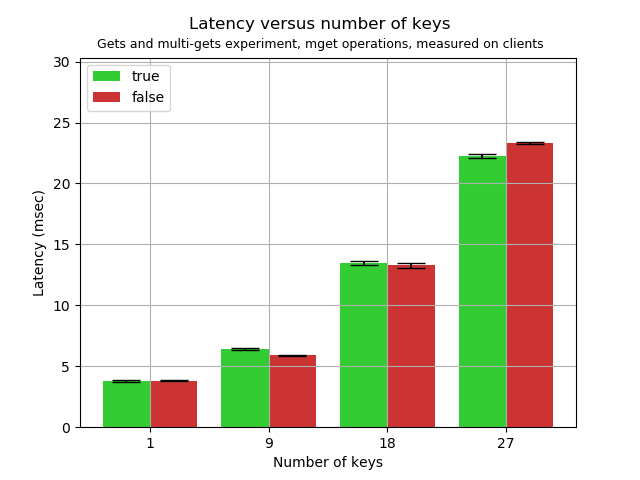
\includegraphics[width=1.0\linewidth ,trim={0 0 0 0},clip]{img/plot/extra-gmg-mget-lat_cli.png}
  \caption{Response times}
  \label{fig:extra-gmg-mget-lat_cli}
\end{subfigure}%
\begin{subfigure}{.5\textwidth}
  \centering
  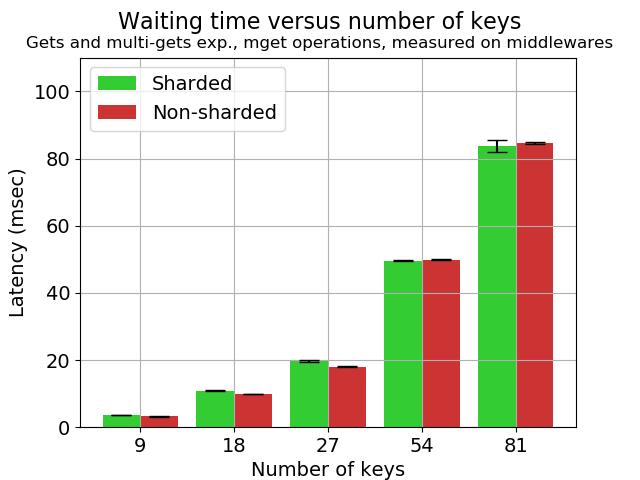
\includegraphics[width=1.0\linewidth ,trim={0 0 0 0},clip]{img/plot/extra-gmg-mget-wtime_mw.png}
  \caption{Server waiting times}
  \label{fig:extra-gmg-mget-wtime_mw}
\end{subfigure}

\begin{subfigure}{.5\textwidth}
  \centering
  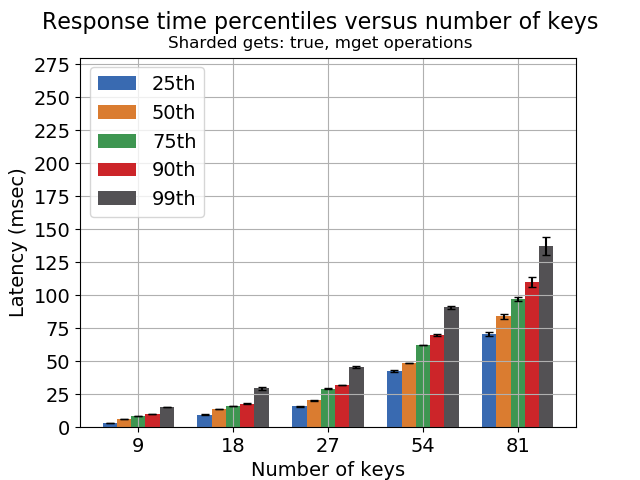
\includegraphics[width=1.0\linewidth ,trim={0 0 0 0},clip]{img/plot/extra-gmg-perc-true.png}
  \caption{Sharded case}
  \label{fig:extra-gmg-perc-true}
\end{subfigure}%
\begin{subfigure}{.5\textwidth}
  \centering
  \includegraphics[width=1.0\linewidth ,trim={0 0 0 0},clip]{img/plot/extra-gmg-perc-false.png}
  \caption{Non-sharded case}
  \label{fig:extra-gmg-perc-false}
\end{subfigure}
\caption{An auxiliary experiment for comparing sharded and non-sharded performances on multi-get requests with bigger key sets. Figures \ref{fig:extra-gmg-mget-lat_cli} and \ref{fig:extra-gmg-mget-wtime_mw} compare the average response time and server waiting time statistics for the sharded and non-sharded reads with 1, 9, 18 and 27 key cases. Figures \ref{fig:extra-gmg-perc-true} and \ref{fig:extra-gmg-perc-false} illustrates 25th, 50th, 75th, 90th and 99th percentiles of sharded and non-sharded reads, for the experiments with aforementioned set of key sizes.}
\label{fig:extra-gmg}
\end{figure}

\section{2K Analysis} \label{sec:2k}
In this section, we perform a $2^{k}$ factorial analysis on three parameters: number of middlewares, number of servers and the number of worker threads per middleware. We believe the effetcs of these parameters are unidirectional, so $2^{k}$ factorial analysis suits our interests best. We solve the linear equation systems for both throughput and response times on both read-only and write-only workloads. Our aim is to assess the impacts of different parameters for different configurations, as well as further investigating and whether an additive or a multiplicative model would capture the interactions and variations in our system best.
\begin{table}[h]
\centering
\begin{tabular}{|l|c|c|c|c|}
\hline 
Parameter & Factor & Variable & {\small Value at min. (-1)} & {\small Value at max. (+1)} \\ 
\hline 
Number of middlewares & A & xA & 1 & 2 \\ 
\hline 
Number of servers & B & xB & 1 & 3 \\ 
\hline 
Worker threads per middleware & C & xC & 8 & 32 \\ 
\hline 
\end{tabular} 
\caption{$2^{k}$ experimental design used in this section, specifying the factors and treatments.} \label{tab:2k-factors}
\end{table}
\par Table \ref{tab:2k-factors} shows the system parameters and their correspoing variables and values chosen for the analyses. For each configurationon each workload, we solve two linear systems, which are illustrated in Equations \ref{eq:add-model} and \ref{eq:mult-model}. The former uses the assumption that the effects of the factors are additive, whereas the latter one assumes multiplicative effects. Multiplicative model is only different from the additive one in the sense that the response variables are logarithms of the observed values. In the scope of this section e denotes error whereas r denotes the number of repetitions.
\begin{footnotesize}
\begin{equation} \label{eq:add-model}
y = q0 + qA*xA + qB*xB + qC*xC + qAB*xA*xB + qBC*xB*xC + qAC*xA*xC + qABC*xA*xB*xC + e
\end{equation}
\begin{equation} \label{eq:mult-model}
log(y) = q0 + qA*xA + qB*xB + qC*xC + qAB*xA*xB + qBC*xB*xC + qAC*xA*xC + qABC*xA*xB*xC + e
\end{equation}
\end{footnotesize}
\par Before going into the results of the analysis, it is good to know how the linear equations are formed and solved. Table \ref{tab:2k-example-table} shows an example of such equation systems, in this case the response variable being the throughput of the system on write-only load. Left part of the table is a sign table where $-1$'s refer to the minimum treatment and $+1$'s refer to the maxiumum treatment for a variable. We always condust our factorial analyses with replications (so-called $2^{k}r$ design) so we solve our equations for the mean response (y\_mean) and estimate the errors in response values as e1, e2 and e3 over three repetitions. After solving the equation system we obtain the effects of the variables (e.g. qA for variable xA or qBC for variable interaction xB*xC) and calculate allocation of variation for each factor through sum of squares values. Equations \ref{eq:ssa}, \ref{eq:sse} and \ref{eq:sst} show how these calculations were done.
\begin{small}
\begin{equation} \label{eq:ssa}
SSA = 2^2*qA^2 \textnormal{, Fraction of variation explained by factor A} = SSA / SST
\end{equation}
\begin{equation} \label{eq:sse}
\textnormal{Sum of Squares for Error: } SSE = \sum_{i=1}^{2^{k}}\sum_{j=1}^{r} e_{ij}^{2}
\end{equation}
\begin{equation} \label{eq:sst}
\textnormal{Total Sum of Squares: } SST = SSA + SSB + SSC + SSAB + SSBC + SSAC + SSABC + SSE
\end{equation}
\end{small}
\begin{table}[h]
\centering
\begin{tabular}{|c|c|c|c|c|c|c|c|c|c|c|c|}
\hline
I & xA & xB & xC & {\small xA*xB} & {\small xB*xC} & {\small xA*xC} & {\small xA*xB*xC} & y\_mean & e1 & e2 & e3 \\ 
\hline
$1$ & $-1$ & $-1$ & $-1$ & $+1$ & $+1$ & $+1$ & $-1$ & 3364.3 & 45.56 & -15.33 & -30.23 \\
\hline
$1$ & $+1$ & $-1$ & $-1$ & $-1$ & $+1$ & $-1$ & $+1$ & 4318.9 & -19.85 & -1.77 & 21.63 \\
\hline
$1$ & $-1$ & $+1$ & $-1$ & $-1$ & $-1$ & $+1$ & $+1$ & 2655.2 & 23.47 & 37.06 & -60.54 \\
\hline
$1$ & $+1$ & $+1$ & $-1$ & $+1$ & $-1$ & $-1$ & $-1$ & 3729.6 & 9.09 & -39.41 & 30.32 \\
\hline
$1$ & $-1$ & $-1$ & $+1$ & $+1$ & $-1$ & $-1$ & $+1$ & 5832.8 & 6.49 & -17.43 & 10.93 \\
\hline
$1$ & $+1$ & $-1$ & $+1$ & $-1$ & $-1$ & $+1$ & $-1$ & 7321.3 & 17.68 & -21.73 & 4.04 \\
\hline
$1$ & $-1$ & $+1$ & $+1$ & $-1$ & $+1$ & $-1$ & $-1$ & 4786.4 & 27.09 & -18.71 & -8.38 \\
\hline
$1$ & $+1$ & $+1$ & $+1$ & $+1$ & $+1$ & $+1$ & $+1$ & 6782.0 & -16.40 & -2.95 & 19.35 \\
\hline
\end{tabular}
\caption{An example system of equations for the $2^{k}$ factorial analyses. Specifically, this set of equations with the corresponding y values model the throughput for the write-only load, assuming additive variable effects. Variable xA, xB and xC denote respectively the effects of number of middlewares, number of servers and the number of worker threads in our model.} \label{tab:2k-example-table}
\end{table}

\change{explain results here, fill the tables} \maybe{The SSE is the unexplained variation attributed to the experimental errors.} \maybe{The logarithmic transformation is useful only if the ratio y max /y min is large. For a small range the log function is almost linear, and so the analysis with the multiplicative model will produce results similar to that with the additive model.}

\begin{table}
\begin{minipage}{.5\textwidth}
\centering
	\begin{tabular}{|c|c|c|}
	\hline 
	{\small Source} & {\small Mean Estimate} & {\small Variation Explained} \\ 
	\hline 
	A & • & • \\ 
	\hline 
	B & • & • \\ 
	\hline 
	C & • & • \\ 
	\hline 
	AB & • & • \\ 
	\hline 
	BC & • & • \\ 
	\hline 
	AC & • & • \\ 
	\hline 
	ABC & • & • \\ 
	\hline 
	Error & • & • \\ 
	\hline 
	Total & • & • \\ 
	\hline 
	\end{tabular} \caption{Throughput analysis, read-only load} \label{tab:2k-tpt-ro}
\end{minipage}%
\begin{minipage}{.5\textwidth}
\centering
	\begin{tabular}{|c|c|c|}
	\hline 
	{\small Source} & {\small Mean Estimate} & {\small Variation Explained} \\ 
	\hline 
	A & • & • \\ 
	\hline 
	B & • & • \\ 
	\hline 
	C & • & • \\ 
	\hline 
	AB & • & • \\ 
	\hline 
	BC & • & • \\ 
	\hline 
	AC & • & • \\ 
	\hline 
	ABC & • & • \\ 
	\hline 
	Error & • & • \\ 
	\hline 
	Total & • & • \\ 
	\hline 
	\end{tabular} \caption{Latency analysis, read-only load} \label{tab:2k-lat-ro}
\end{minipage}
\end{table}\label{tab:2k-ro}

\begin{table}
\begin{minipage}{.5\textwidth}
\centering
	\begin{tabular}{|c|c|c|}
	\hline 
	{\small Source} & {\small Mean Estimate} & {\small Variation Explained} \\ 
	\hline 
	A & • & • \\ 
	\hline 
	B & • & • \\ 
	\hline 
	C & • & • \\ 
	\hline 
	AB & • & • \\ 
	\hline 
	BC & • & • \\ 
	\hline 
	AC & • & • \\ 
	\hline 
	ABC & • & • \\ 
	\hline 
	Error & • & • \\ 
	\hline 
	Total & • & • \\ 
	\hline 
	\end{tabular} \caption{Throughput analysis, write-only load} \label{tab:2k-tpt-wo}
\end{minipage}%
\begin{minipage}{.5\textwidth}
\centering
	\begin{tabular}{|c|c|c|}
	\hline 
	{\small Source} & {\small Mean Estimate} & {\small Variation Explained} \\ 
	\hline 
	A & • & • \\ 
	\hline 
	B & • & • \\ 
	\hline 
	C & • & • \\ 
	\hline 
	AB & • & • \\ 
	\hline 
	BC & • & • \\ 
	\hline 
	AC & • & • \\ 
	\hline 
	ABC & • & • \\ 
	\hline 
	Error & • & • \\ 
	\hline 
	Total & • & • \\ 
	\hline 
	\end{tabular} \caption{Latency analysis, write-only load} \label{tab:2k-lat-wo}
\end{minipage}
\end{table}\label{tab:2k-wo}

\section{Queuing Model} \label{sec:queueing-model}

\subsection{M/M/1} \label{sec:mm1}

\subsection{M/M/m} \label{sec:mmm}

\subsection{Network of Queues} \label{sec:network-of-queues}
\maybe{You need to consider both 1 and 2 middleware configuration. You need to analyze both read only and write only workloads. You can set the number of worker threads to the constant that delivers highest throughput.}

\begin{thebibliography}{9}
\bibitem{memcached} Memcached: a distributed memory object caching system \url{https://memcached.org/}
\bibitem{memtier} memtier\_benchmark: a high-throughput benchmarking tool for Redis \& Memcached \url{https://github.com/RedisLabs/memtier\_benchmark}
\bibitem{dstat} Dstat: a versatile resource statistics tool \url{http://dag.wiee.rs/home-made/dstat/}
\bibitem{cssh} Cluster SSH: cluster administration tool via SSH \url{https://github.com/duncs/clusterssh}
\bibitem{iperf} iPerf: the TCP, UDP and SCTP network bandwidth measurement tool \url{https://iperf.fr/}
\end{thebibliography}

\end{document}
